%==============================================================
%  ĐỒ ÁN TỐT NGHIỆP
%  Path Tracer thời gian thực tăng tốc bằng CUDA
%  Biên dịch bằng: XeLaTeX (hỗ trợ tiếng Việt)
%    xelatex main.tex  (chạy 2-3 lần để cập nhật mục lục)
%  hoặc dùng script:
%    bash compile_latex.sh report/main.tex --engine xelatex --preview
%==============================================================
\documentclass[12pt,a4paper,oneside]{report}

%------------------- Font & Ngôn ngữ -------------------
\usepackage{fontspec}
\setmainfont{Times New Roman}             % font hệ thống Windows, hỗ trợ tiếng Việt
\usepackage[vietnamese]{babel}

%------------------- Hình học trang -------------------
\usepackage{geometry}
\geometry{a4paper, top=2.5cm, bottom=2.5cm, left=3cm, right=2cm}

%------------------- Các gói thường dùng -------------------
\usepackage{graphicx}
\usepackage{float}
\usepackage{xcolor}
\usepackage{amsmath,amssymb}
\usepackage{booktabs}
\usepackage{tabularx}
\usepackage{enumitem}
\usepackage{titlesec}
\usepackage{caption}
\usepackage{subcaption}
\usepackage{listings}
\usepackage{setspace}
\onehalfspacing                          % giãn dòng 1.5

%------------------- Vẽ hình (TikZ / pgfplots) -------------------
\usepackage{tikz}
\usepackage{pgfplots}
\pgfplotsset{compat=1.18}
\usetikzlibrary{arrows.meta, calc, decorations.pathmorphing, patterns, angles,
                quotes, positioning, shapes.geometric}

%------------------- Mục lục & liên kết -------------------
\usepackage[hidelinks]{hyperref}
\hypersetup{
  colorlinks=false,
  pdftitle={Path Tracer thoi gian thuc tang toc bang CUDA},
  pdfauthor={Nguyen Xuan Khoi}
}

%------------------- Định dạng tiêu đề chương -------------------
\titleformat{\chapter}[display]
  {\normalfont\huge\bfseries}{\chaptertitlename\ \thechapter}{18pt}{\Huge}
\titlespacing*{\chapter}{0pt}{0pt}{30pt}

%------------------- Cấu hình listings (mã nguồn) -------------------
\definecolor{codegray}{gray}{0.95}
\definecolor{codekw}{rgb}{0.0,0.3,0.6}
\definecolor{codecomment}{rgb}{0.0,0.5,0.0}
\lstset{
  backgroundcolor=\color{codegray},
  basicstyle=\ttfamily\footnotesize,
  keywordstyle=\color{codekw}\bfseries,
  commentstyle=\color{codecomment}\itshape,
  breaklines=true,
  frame=single,
  numbers=left,
  numberstyle=\tiny,
  showstringspaces=false,
  captionpos=b
}

%==============================================================
\begin{document}

%--------- TRANG 1: TRANG BÌA ---------
% !TEX root = main.tex
%==============================================================
%  TRANG BÌA - theo mẫu Đại học Bách Khoa Hà Nội
%==============================================================
\begin{titlepage}
\centering
\thispagestyle{empty}

{\large\bfseries TRƯỜNG ĐẠI HỌC BÁCH KHOA HÀ NỘI\par}

\vspace{2.5cm}

{\fontsize{30}{36}\selectfont\bfseries ĐỒ ÁN II\par}

\vspace{1.0cm}

{\large\bfseries Path Tracing Renderer with CUDA\par}

\vspace{1.2cm}

{\large\bfseries NGUYỄN XUÂN KHÔI\par}
{\normalsize MSSV: 20225022\par}
{\normalsize khoi.nx225022@sis.hust.edu.vn\par}

\vspace{3.0cm}

% Khối thông tin căn trái
\begin{flushleft}
\hspace{1.5cm}
\begin{tabular}{@{}p{4.5cm}p{7cm}@{}}
\textbf{Giảng viên hướng dẫn:} & ThS. Nguyễn Duy Hiệp \hrulefill \\[0.2cm]
                               & \hfill \textit{Chữ kí GVHD} \\[0.8cm]
\textbf{Khoa:}                 & Khoa học máy tính \\[0.4cm]
\textbf{Trường:}               & Công nghệ Thông tin và Truyền thông \\
\end{tabular}
\end{flushleft}

\vfill

{\bfseries HÀ NỘI, 06/2026\par}

\vspace{1cm}
\end{titlepage}


%--------- PHẦN ĐẦU (Front matter) ---------
\cleardoublepage
\pagenumbering{roman}
% !TEX root = ../main.tex
%==============================================================
%  LỜI CẢM ƠN
%==============================================================
\thispagestyle{empty}
\begin{center}
{\Large\bfseries LỜI CẢM ƠN}
\end{center}
\vspace{1cm}

Đồ án này là kết quả của quá trình học tập, nghiên cứu và thực hành của bản thân
tôi trong suốt thời gian qua. Để hoàn thành được đồ án, bên cạnh nỗ lực của cá
nhân, tôi đã nhận được rất nhiều sự giúp đỡ và động viên từ thầy cô, gia đình và
bạn bè.

Trước hết, tôi xin bày tỏ lòng biết ơn sâu sắc tới thầy giáo hướng dẫn, TS. Ngô
Thành Trung. Thầy không chỉ truyền đạt những kiến thức nền tảng quý báu về đồ họa
máy tính và tính toán song song, mà còn định hướng tư duy, kiên nhẫn góp ý và tạo
điều kiện để tôi tự do theo đuổi ý tưởng của mình. Nếu không có sự hướng dẫn tận
tình của thầy, đồ án này khó có thể hoàn thành.

Tôi cũng xin gửi lời cảm ơn chân thành tới các thầy cô trong Trường Công nghệ
Thông tin và Truyền thông, Đại học Bách Khoa Hà Nội, vì những kiến thức và kinh
nghiệm đã trang bị cho tôi trong suốt quá trình học tập.

Cuối cùng, tôi xin cảm ơn gia đình và bạn bè -- những người đã luôn ở bên cạnh,
ủng hộ và là điểm tựa tinh thần vững chắc cho tôi trong những lúc khó khăn nhất.

Tôi xin chân thành cảm ơn!

\cleardoublepage
% !TEX root = ../main.tex
%==============================================================
%  LỜI CAM KẾT
%==============================================================
\thispagestyle{empty}
\begin{center}
{\Large\bfseries LỜI CAM KẾT}
\end{center}
\vspace{0.8cm}

\noindent Họ và tên sinh viên: Nguyễn Xuân Khôi \dotfill{}\\[0.4cm]
\noindent Mã số sinh viên: 20225022 \dotfill{}\\[0.4cm]
\noindent Điện thoại liên lạc: \dotfill{}\\[0.4cm]
\noindent Email: khoi.nx225022@sis.hust.edu.vn \dotfill{}\\[0.4cm]
\noindent Lớp: \dotfill{}\\[0.4cm]
\noindent Hệ đào tạo: \dotfill{}\\[1.0cm]

Tôi -- Nguyễn Xuân Khôi -- cam kết Đồ án II là công trình nghiên cứu của bản thân
tôi dưới sự hướng dẫn của ThS. Nguyễn Duy Hiệp. Các kết quả nêu trong đồ án là
trung thực, là thành quả của riêng tôi, không sao chép theo bất kỳ công trình nào
khác. Tất cả những tham khảo trong đồ án -- bao gồm hình ảnh, bảng biểu, số liệu
và các câu từ trích dẫn -- đều được ghi rõ ràng và đầy đủ nguồn gốc trong danh
mục tài liệu tham khảo. Tôi xin hoàn toàn chịu trách nhiệm với dù chỉ một sao
chép vi phạm quy chế của nhà trường.

\vspace{1.0cm}
\begin{flushright}
\textit{Hà Nội, ngày\quad tháng\quad năm 2026}\\[0.3cm]
Tác giả đồ án\\[1.5cm]
\textit{Nguyễn Xuân Khôi}
\end{flushright}

\cleardoublepage
% !TEX root = ../main.tex
%==============================================================
%  TÓM TẮT NỘI DUNG ĐỒ ÁN
%==============================================================
\thispagestyle{empty}
\begin{center}
{\Large\bfseries TÓM TẮT NỘI DUNG ĐỒ ÁN}
\end{center}
\vspace{1cm}

Hình ảnh được sinh từ máy tính đóng vai trò quan trọng trong nhiều ứng dụng của
thế giới thực, từ lĩnh vực giải trí như điện ảnh, trò chơi điện tử đến các lĩnh
vực kỹ thuật như kiến trúc và y học. Kết xuất dựa trên vật lý (physically based
rendering) là lớp giải thuật mã hóa các định luật truyền ánh sáng thành mô hình
toán học để tạo ra hình ảnh có độ chân thực cao. Trong số đó, Path Tracing là
phương pháp tổng quát và chính xác, song có chi phí tính toán rất lớn do phải mô
phỏng đường đi của hàng triệu tia sáng bằng tích phân Monte Carlo, dẫn tới thời
gian kết xuất kéo dài và khó đạt tốc độ tương tác.

Trong đồ án này, tôi nghiên cứu và xây dựng một bộ kết xuất Path Tracing chạy
song song trên kiến trúc CUDA của NVIDIA nhằm khai thác sức mạnh của GPU để đạt
tốc độ kết xuất thời gian thực. Hệ thống hiện thực đầy đủ chu trình dò tia trên
GPU, bao gồm: thuật toán Path Tracing với tích lũy theo thời gian và khử răng
cưa; hệ thống vật liệu khuếch tán, kim loại và điện môi; mô hình camera thấu kính
mỏng với hiệu ứng độ sâu trường ảnh và nhòe chuyển động; cơ chế cầu nối
CUDA--OpenGL cho phép hiển thị trực tiếp từ bộ nhớ video; cùng bộ nạp cảnh theo
định dạng Mitsuba~3 và giao diện điều khiển tương tác.

Kết quả cho thấy hệ thống có khả năng kết xuất các cảnh thử nghiệm ở tốc độ
tương tác, đồng thời hội tụ dần về hình ảnh ít nhiễu khi camera giữ nguyên. Đồ án
cũng chỉ ra các hướng tối ưu và mở rộng trong tương lai như cấu trúc tăng tốc BVH
và các kỹ thuật giảm nhiễu nâng cao.

\vspace{1.5cm}
\begin{flushright}
Sinh viên thực hiện\\[0.3cm]
\textit{(Ký và ghi rõ họ tên)}
\end{flushright}

\cleardoublepage
% !TEX root = ../main.tex
%==============================================================
%  ABSTRACT (English)
%==============================================================
\thispagestyle{empty}
\begin{center}
{\Large\bfseries ABSTRACT}
\end{center}
\vspace{1cm}

Computer-generated images play an important role in many real-world applications,
ranging from recreational fields such as cinema and video games to engineering
fields such as architecture and medicine. Physically based rendering is the class
of algorithms that codifies the physical laws of light transport into mathematical
models in order to produce highly realistic images. Among these, Path Tracing is a
general and accurate method, but it is computationally expensive because it must
simulate the paths of millions of light rays through Monte Carlo integration,
resulting in long rendering times and making interactive frame rates difficult to
achieve.

In this project, I study and build a Path Tracer that runs in parallel on NVIDIA's
CUDA architecture to exploit the computational power of the GPU and achieve
real-time rendering. The system implements the complete ray tracing pipeline on the
GPU, including: the Path Tracing algorithm with temporal accumulation and
anti-aliasing; a material system supporting diffuse, metallic, and dielectric
surfaces; a thin-lens camera model with depth-of-field and motion-blur effects; a
CUDA--OpenGL interoperability mechanism that enables display directly from video
memory; together with a Mitsuba~3 scene loader and an interactive control interface.

Experimental results show that the system is able to render the test scenes at
interactive rates while progressively converging to a low-noise image when the
camera remains static. The project also identifies future optimization and
extension directions, such as bounding volume hierarchy (BVH) acceleration
structures and advanced denoising techniques.

\vspace{1.5cm}
\begin{flushright}
Student\\[0.3cm]
\textit{(Signature and full name)}
\end{flushright}


%--------- MỤC LỤC ---------
\cleardoublepage
\tableofcontents
\listoffigures

%--------- NỘI DUNG CHÍNH ---------
\cleardoublepage
\pagenumbering{arabic}

% !TEX root = ../main.tex
%==============================================================
\chapter{Giới thiệu đề tài}
\label{ch:gioi-thieu}

\section{Đặt vấn đề}
Kết xuất đồ họa (rendering) là quá trình tạo ra hình ảnh hai chiều từ mô tả
của một cảnh ba chiều. Trong số các kỹ thuật kết xuất, \textit{Path Tracing}
là phương pháp dựa trên mô phỏng vật lý của ánh sáng, cho phép tạo ra hình ảnh
có độ chân thực cao với các hiệu ứng như phản xạ, khúc xạ, đổ bóng mềm và
chiếu sáng toàn cục (global illumination). Tuy nhiên, chi phí tính toán của
Path Tracing rất lớn do phải mô phỏng hàng triệu tia sáng cho mỗi khung hình.

% TODO: Bổ sung dẫn nhập về nhu cầu kết xuất thời gian thực.

\section{Mục tiêu của đề tài}
Đề tài hướng tới việc nghiên cứu và xây dựng một bộ kết xuất Path Tracing
chạy song song trên kiến trúc CUDA của NVIDIA nhằm đạt tốc độ tương tác
(thời gian thực). Các mục tiêu cụ thể bao gồm:
\begin{itemize}[noitemsep]
  \item Hiện thực thuật toán Path Tracing trên GPU bằng CUDA.
  \item Xây dựng hệ thống vật liệu Lambertian, Metal, Dielectric và camera vật lý
        có độ sâu trường ảnh, nhòe chuyển động.
  \item Hiển thị thời gian thực qua cầu nối CUDA--OpenGL và tích lũy mẫu theo
        thời gian để khử nhiễu.
  \item Nạp cảnh theo định dạng Mitsuba 3 và cung cấp giao diện điều khiển tương tác.
\end{itemize}

\section{Phạm vi và đối tượng nghiên cứu}
% TODO: Mô tả phạm vi (loại cảnh hỗ trợ, định dạng nhập, phần cứng thử nghiệm).

\section{Cấu trúc báo cáo}
Báo cáo được tổ chức thành năm chương. Chương~\ref{ch:gioi-thieu} giới thiệu đề tài.
Chương~\ref{ch:ly-thuyet} trình bày nền tảng lý thuyết. Chương~\ref{ch:trien-khai}
mô tả quá trình triển khai hệ thống. Chương~\ref{ch:danh-gia} trình bày kết quả
và đánh giá. Chương~\ref{ch:ket-luan} đưa ra kết luận và hướng phát triển.

% !TEX root = ../main.tex
%==============================================================
\chapter{Nền tảng lý thuyết}
\label{ch:ly-thuyet}

Chương này trình bày cơ sở lý thuyết của hệ thống. Trước hết ta xây dựng các đại
lượng trắc quang (radiometry) và phương trình kết xuất mô tả sự cân bằng năng
lượng ánh sáng. Tiếp theo là phương pháp Monte Carlo dùng để ước lượng tích phân
trong phương trình đó, kèm các kỹ thuật giảm phương sai. Phần sau trình bày mô
hình hàm phản xạ (BRDF) cho ba loại vật liệu được hiện thực, mô hình camera thấu
kính mỏng, bài toán tìm giao tia--vật thể, và cuối cùng là mô hình tính toán song
song trên CUDA. Nội dung được tham khảo chủ yếu từ loạt sách \emph{Ray Tracing in
One Weekend}~\cite{shirley2020raytracing, shirley2020restoflife} và sách
\emph{Physically Based Rendering}~\cite{pharr2016pbrt}.

\section{Đại lượng trắc quang và phương trình kết xuất}

\subsection{Góc khối và bức xạ}
Để định lượng ánh sáng một cách độc lập với hình học, ta dùng khái niệm \emph{góc
khối} (solid angle). Một vùng trên mặt cầu đơn vị chắn bởi một hướng nhìn có độ
lớn góc khối $d\omega$ (đơn vị steradian). Trong hệ tọa độ cầu, vi phân góc khối
quanh hướng $(\theta,\phi)$ là
\begin{equation}
d\omega = \sin\theta\, d\theta\, d\phi .
\end{equation}

Đại lượng trung tâm của kết xuất dựa trên vật lý là \emph{bức xạ} (radiance)
$L$: công suất ánh sáng trên một đơn vị diện tích vuông góc, trên một đơn vị góc
khối, ký hiệu $L(\mathbf{p}, \omega)$ tại điểm $\mathbf{p}$ theo hướng $\omega$
\cite{pharr2016pbrt}. Bức xạ là đại lượng được \emph{bảo toàn dọc theo tia} trong
môi trường chân không và là giá trị mà mỗi tia trong path tracer mang theo. Từ
bức xạ tới, \emph{độ rọi} (irradiance) $E$ trên một bề mặt có pháp tuyến
$\mathbf{n}$ thu được bằng cách lấy tích phân theo bán cầu, có trọng số cosine:
\begin{equation}
\label{eq:irradiance}
E(\mathbf{p}) = \int_{\Omega} L_i(\mathbf{p}, \omega_i)\,
                (\omega_i \cdot \mathbf{n})\, d\omega_i .
\end{equation}
Thừa số cosine $(\omega_i\cdot\mathbf{n})=\cos\theta_i$ phản ánh việc một chùm
sáng tới xiên trải năng lượng trên diện tích lớn hơn nên đóng góp ít hơn.

\begin{figure}[H]
\centering
\begin{tikzpicture}[scale=1.7,>=Stealth]
  % surface
  \fill[gray!12] (-1.7,-0.35) rectangle (1.7,0);
  \draw[thick] (-1.7,0) -- (1.7,0);
  \foreach \x in {-1.5,-1.2,...,1.5}
    \draw[gray] (\x,0) -- (\x-0.18,-0.18);
  % hemisphere
  \draw[dashed,gray!70] (-1.4,0) arc (180:0:1.4);
  % point
  \coordinate (p) at (0,0);
  % normal
  \draw[->,thick] (p) -- (0,1.5) node[above]{$\mathbf{n}$};
  % incoming ray
  \draw[->,thick,blue!70!black] (-1.19,1.19) -- (p);
  \node[blue!70!black] at (-1.0,1.32) {$\omega_i$};
  % outgoing ray
  \draw[->,thick,red!75!black] (p) -- (1.19,1.19);
  \node[red!75!black] at (1.0,1.32) {$\omega_o$};
  % theta_i angle
  \draw (0,0.55) arc (90:135:0.55);
  \node at (-0.18,0.72) {\scriptsize$\theta_i$};
  % solid angle patch
  \draw[fill=blue!15,draw=blue!50] (-0.92,0.92) ++(-0.12,0.05)
        arc (135:120:1.4) -- ++(0.1,0.13) arc (120:135:1.55) -- cycle;
  \node[blue!60!black] at (-1.05,0.62) {\scriptsize$d\omega_i$};
  \fill (p) circle (1.1pt);
  \node[below=2pt] at (p) {$\mathbf{p}$};
\end{tikzpicture}
\caption{Hình học tại một điểm bề mặt: bức xạ tới theo hướng $\omega_i$ trong góc
khối vi phân $d\omega_i$, bức xạ phản xạ theo hướng $\omega_o$, với pháp tuyến
$\mathbf{n}$ và góc tới $\theta_i$.}
\label{fig:hemisphere}
\end{figure}

\subsection{Hàm phản xạ lưỡng hướng (BRDF)}
Cách một bề mặt phản xạ ánh sáng được mô tả bởi \emph{hàm phân bố phản xạ lưỡng
hướng} (Bidirectional Reflectance Distribution Function -- BRDF), định nghĩa là
tỉ số giữa bức xạ phản xạ theo hướng $\omega_o$ và độ rọi vi phân tới từ hướng
$\omega_i$:
\begin{equation}
f_r(\mathbf{p}, \omega_i, \omega_o) =
   \frac{dL_o(\mathbf{p}, \omega_o)}{L_i(\mathbf{p}, \omega_i)\,
   (\omega_i \cdot \mathbf{n})\, d\omega_i} .
\end{equation}
Một BRDF hợp lệ về mặt vật lý phải thỏa mãn hai tính chất: \emph{tính đối xứng
Helmholtz} $f_r(\omega_i,\omega_o)=f_r(\omega_o,\omega_i)$, và \emph{bảo toàn
năng lượng} -- tổng năng lượng phản xạ không vượt quá năng lượng tới
\cite{pharr2016pbrt}.

\subsection{Phương trình kết xuất}
Kết hợp BRDF với độ rọi tới, bức xạ rời khỏi điểm $\mathbf{p}$ theo hướng
$\omega_o$ được cho bởi \emph{phương trình kết xuất} do Kajiya đề
xuất~\cite{kajiya1986rendering}:
\begin{equation}
\label{eq:rendering}
L_o(\mathbf{p}, \omega_o) = L_e(\mathbf{p}, \omega_o)
  + \int_{\Omega} f_r(\mathbf{p}, \omega_i, \omega_o)\,
    L_i(\mathbf{p}, \omega_i)\, (\omega_i \cdot \mathbf{n})\, d\omega_i,
\end{equation}
trong đó $L_e$ là bức xạ tự phát (vật liệu phát sáng), số hạng tích phân là bức
xạ phản xạ. Đây là phương trình \emph{Fredholm loại hai}: ẩn $L$ xuất hiện ở cả
hai vế vì bức xạ tới $L_i(\mathbf{p},\omega_i)$ tại $\mathbf{p}$ chính là bức xạ
đi ra $L_o(\mathbf{p}', -\omega_i)$ của điểm $\mathbf{p}'$ mà tia $(\mathbf{p},
\omega_i)$ chạm tới. Tính đệ quy này khiến lời giải giải tích là bất khả thi với
cảnh tổng quát, do đó cần phương pháp số.

\section{Ước lượng Monte Carlo}

\subsection{Bộ ước lượng cơ bản}
Phương pháp Monte Carlo xấp xỉ một tích phân xác định bằng kỳ vọng thống kê. Với
tích phân $I = \int g(x)\, dx$, nếu lấy $N$ mẫu độc lập $x_k$ theo mật độ xác
suất $p(x)$ (với $p(x)>0$ ở những nơi $g(x)\neq0$), \emph{bộ ước lượng Monte
Carlo} là
\begin{equation}
\label{eq:montecarlo}
\langle I \rangle = \frac{1}{N}\sum_{k=1}^{N} \frac{g(x_k)}{p(x_k)} .
\end{equation}
Bộ ước lượng này \emph{không chệch} (unbiased): $\mathbb{E}[\langle I\rangle]=I$
với mọi $N$. Phương sai của nó giảm tỉ lệ $1/N$, nên \emph{sai số chuẩn} (độ lệch
chuẩn) giảm theo $O(1/\sqrt{N})$. Hệ quả thực tiễn: muốn giảm một nửa nhiễu cần
gấp bốn lần số mẫu -- đây là nguồn gốc của hiện tượng \emph{nhiễu hạt} (noise)
đặc trưng và chi phí tính toán lớn của path tracing~\cite{shirley2020restoflife}.

\subsection{Lấy mẫu theo tầm quan trọng}
Phương sai phụ thuộc mạnh vào mức độ phù hợp giữa $p(x)$ và $g(x)$. Nếu chọn
$p(x)$ tỉ lệ với $g(x)$ thì tỉ số $g/p$ gần như hằng số và phương sai giảm mạnh;
đây là ý tưởng \emph{lấy mẫu theo tầm quan trọng} (importance
sampling)~\cite{veach1997robust}. Trong kết xuất, do tích phân
\eqref{eq:rendering} chứa thừa số cosine và BRDF, ta thường lấy mẫu hướng
$\omega_i$ theo phân bố cosine hoặc theo hình dạng của BRDF thay vì đều trên bán
cầu. Hệ thống hiện tại lấy mẫu khuếch tán theo phân bố cosine (Mục~\ref{sec:vatlieu});
việc lấy mẫu trực tiếp nguồn sáng (Next Event Estimation) là hướng mở rộng nêu ở
Chương~\ref{ch:ket-luan}.

\subsection{Công thức tích phân đường và hệ số suy giảm}
Khai triển đệ quy phương trình \eqref{eq:rendering} cho \emph{công thức tích phân
đường} (path integral): bức xạ tới camera là tổng đóng góp của mọi đường ánh sáng
nối nguồn sáng tới mắt qua một số lần phản xạ. Path tracing ước lượng tổng này
bằng cách, tại mỗi điểm va chạm, lấy \emph{một} hướng tán xạ ngẫu nhiên và lần
theo tia đó -- tạo thành một đường đi ngẫu nhiên. Đóng góp của đường được tích
lũy qua \emph{hệ số suy giảm} (throughput) $\beta$, cập nhật nhân dồn sau mỗi va
chạm:
\begin{equation}
\label{eq:throughput}
\beta_n = \beta_{n-1}\,
          \frac{f_r(\mathbf{p}_n,\omega_i,\omega_o)\,(\omega_i\cdot\mathbf{n})}
               {p(\omega_i)},
\qquad \beta_0 = 1 .
\end{equation}
Khi tia thoát khỏi cảnh và gặp nguồn sáng nền, bức xạ thu được bằng tích của bức
xạ nền với $\beta$. Với cách lấy mẫu khuếch tán theo cosine, thừa số cosine và
mẫu số $p(\omega_i)$ triệt tiêu nhau, khiến việc cập nhật $\beta$ rút gọn về phép
nhân với albedo -- đúng như hiện thực trong mã nguồn (Chương~\ref{ch:trien-khai}).

\begin{figure}[H]
\centering
\begin{tikzpicture}[scale=1.0,>=Stealth,
   surf/.style={line width=1.2pt,gray!70}]
  % camera
  \node[draw,fill=gray!10,minimum width=0.7cm,minimum height=0.5cm] (cam) at (0,0) {};
  \node[below=1pt of cam,font=\small] {Camera};
  % bounce points
  \coordinate (b1) at (2.3,0.9);
  \coordinate (b2) at (4.4,-0.4);
  \coordinate (b3) at (6.2,1.1);
  % surfaces (short segments) with normals
  \draw[surf] ($(b1)+(-0.45,-0.25)$) -- ($(b1)+(0.45,0.25)$);
  \draw[surf] ($(b2)+(-0.5,0.1)$) -- ($(b2)+(0.5,-0.1)$);
  \draw[surf] ($(b3)+(-0.4,-0.3)$) -- ($(b3)+(0.4,0.3)$);
  % light source
  \node[star,star points=8,star point ratio=0.6,fill=yellow!80!orange,
        draw=orange,minimum size=0.9cm] (L) at (7.8,2.3) {};
  \node[above=0pt of L,font=\small] {Nguồn sáng};
  % path segments
  \draw[->,thick,blue!70!black] (cam.east) -- (b1) node[midway,above,font=\scriptsize]{$\beta_0$};
  \draw[->,thick,blue!70!black] (b1) -- (b2) node[midway,above,font=\scriptsize]{$\beta_1$};
  \draw[->,thick,blue!70!black] (b2) -- (b3) node[midway,below,font=\scriptsize]{$\beta_2$};
  \draw[->,thick,blue!70!black] (b3) -- (L) node[midway,above left,font=\scriptsize]{$\beta_3$};
  % bounce dots
  \foreach \b in {b1,b2,b3} \fill (\b) circle (1.6pt);
  \node[right=1pt,font=\scriptsize] at (b1) {$\mathbf{p}_1$};
  \node[right=1pt,font=\scriptsize] at (b2) {$\mathbf{p}_2$};
  \node[right=1pt,font=\scriptsize] at (b3) {$\mathbf{p}_3$};
\end{tikzpicture}
\caption{Một đường đi ngẫu nhiên trong Path Tracing: tia xuất phát từ camera, tán
xạ qua các điểm va chạm $\mathbf{p}_1,\mathbf{p}_2,\dots$ và kết thúc tại nguồn
sáng; hệ số suy giảm $\beta$ được nhân dồn dọc theo đường.}
\label{fig:pathtrace}
\end{figure}

\subsection{Kết thúc đường đi và Russian Roulette}
Vì một đường có thể phản xạ vô hạn, cần điều kiện dừng. Cách đơn giản là giới hạn
độ sâu tối đa, song điều này tạo ra sai lệch (bias) do bỏ qua các đường dài. Một
giải pháp không chệch là \emph{Russian Roulette}~\cite{pharr2016pbrt}: tại mỗi
bước, kết thúc đường với xác suất $q$ và chia phần còn lại cho $1-q$ để giữ kỳ
vọng không đổi. Hệ thống áp dụng giới hạn độ sâu (tối đa 50 lần dội) kết hợp dừng
sớm khi $\beta$ suy giảm gần bằng 0 -- một xấp xỉ thực dụng cho chế độ thời gian
thực.

\section{Lấy mẫu điểm ảnh và tích lũy theo thời gian}

\subsection{Lý thuyết lấy mẫu và hiện tượng răng cưa}
Quá trình tạo ảnh số thực chất là \emph{lấy mẫu} (sampling) một hàm ảnh liên tục
$f(x,y)$ -- giá trị bức xạ tại mọi điểm trên mặt phẳng ảnh -- tại một lưới điểm
ảnh rời rạc, rồi \emph{tái dựng} (reconstruction) ảnh hiển thị từ các mẫu đó. Cơ
sở lý thuyết của quá trình này là phân tích Fourier~\cite{pharr2016pbrt}.

Mỗi hàm $f$ có một \emph{phổ tần số} $F = \mathcal{F}\{f\}$ thu được qua biến đổi
Fourier. Việc lấy mẫu đều với bước $T$ tương đương nhân $f$ với một chuỗi xung
Dirac (Dirac comb) khoảng cách $T$. Theo định lý tích chập, trong miền tần số
phép nhân này trở thành tích chập của phổ $F$ với một chuỗi xung khoảng cách
$1/T$, tạo ra \emph{vô số bản sao} của phổ gốc lặp lại theo chu kỳ $1/T$:
\begin{equation}
\mathcal{F}\Big\{ f \cdot \textstyle\sum_n \delta(x - nT)\Big\}
   = F * \frac{1}{T}\sum_k \delta\!\Big(\nu - \frac{k}{T}\Big).
\end{equation}
Để khôi phục $f$, ta lọc lấy bản sao trung tâm bằng một bộ lọc thông thấp lý
tưởng. Điều này khả thi \emph{nếu và chỉ nếu} các bản sao không chồng lấn, tức
hàm phải \emph{giới hạn dải tần} (band-limited) với tần số lớn nhất $\nu_{\max}$,
và tần số lấy mẫu thỏa
\begin{equation}
\label{eq:nyquist}
\frac{1}{T} \;>\; 2\,\nu_{\max} .
\end{equation}
Bất đẳng thức~\eqref{eq:nyquist} chính là \emph{định lý lấy mẫu
Nyquist--Shannon}; ngưỡng $2\nu_{\max}$ gọi là \emph{tần số Nyquist}.

Trong kết xuất, điều kiện này gần như luôn bị vi phạm: biên hình học, bóng đổ
sắc nét hay hoa văn texture tạo ra các \emph{bước nhảy} có phổ trải tới vô hạn
nên ảnh \emph{không} giới hạn dải tần. Khi đó các bản sao phổ chồng lấn, năng
lượng tần số cao ``giả dạng'' thành tần số thấp sau khi tái dựng, sinh ra các
sai lệch nhìn thấy được gọi là \emph{răng cưa} (aliasing): biên xiên bị bậc
thang, hoa văn nhỏ biến thành vân moiré.

\begin{figure}[H]
\centering
\begin{tikzpicture}[scale=1.0,>=Stealth]
  % ---- top: adequate sampling ----
  \begin{scope}[yshift=2.2cm]
    \draw[->] (-3.2,0) -- (3.2,0) node[right,font=\scriptsize]{$\nu$};
    \foreach \c in {-2,0,2} {
      \draw[blue!60!black,fill=blue!12] (\c-0.7,0) -- (\c,0.8) -- (\c+0.7,0) -- cycle;
    }
    \node[font=\scriptsize] at (0,1.0) {phổ gốc};
    \node[font=\scriptsize,gray] at (2.1,0.95) {bản sao};
    \node[left,font=\scriptsize] at (-3.2,0.55) {(a)};
  \end{scope}
  % ---- bottom: undersampling -> overlap ----
  \begin{scope}
    \draw[->] (-3.2,0) -- (3.2,0) node[right,font=\scriptsize]{$\nu$};
    \foreach \c in {-1.1,0,1.1} {
      \draw[red!60!black,fill=red!12] (\c-0.7,0) -- (\c,0.8) -- (\c+0.7,0) -- cycle;
    }
    % overlap markers
    \fill[red!45,opacity=0.6] (-0.55,0) -- (-0.55,0.2) -- (-0.4,0) -- cycle;
    \fill[red!45,opacity=0.6] (0.55,0) -- (0.55,0.2) -- (0.4,0) -- cycle;
    \node[font=\scriptsize,red!70!black] at (0.0,1.0) {vùng chồng lấn $\to$ răng cưa};
    \node[left,font=\scriptsize] at (-3.2,0.55) {(b)};
  \end{scope}
\end{tikzpicture}
\caption{Phổ tần số sau khi lấy mẫu gồm phổ gốc và các bản sao lặp lại. (a) Khi
thỏa điều kiện Nyquist~\eqref{eq:nyquist}, các bản sao tách rời nên khôi phục
được tín hiệu. (b) Khi lấy mẫu thiếu (hoặc tín hiệu không giới hạn dải tần), các
bản sao chồng lấn, gây hiện tượng răng cưa.}
\label{fig:nyquist}
\end{figure}

\subsection{Khử răng cưa bằng lấy mẫu ngẫu nhiên}
Có hai hướng chống răng cưa. Hướng thứ nhất là \emph{tiền lọc} (prefiltering) --
làm mượt hàm ảnh để giới hạn dải tần trước khi lấy mẫu -- nhưng nhìn chung không
khả thi vì hàm ảnh không có dạng giải tích. Hướng thứ hai, thực dụng hơn, là
\emph{tăng tần số lấy mẫu}: bắn nhiều tia trên mỗi điểm ảnh (\emph{siêu lấy mẫu},
supersampling) để đẩy tần số Nyquist lên cao, thu hẹp vùng bị răng cưa.

Điều quan trọng là path tracer dùng \emph{lấy mẫu ngẫu nhiên} (stochastic
sampling) thay vì lưới đều. Với mẫu đều, năng lượng tần số cao chồng lấn tạo ra
các vân răng cưa có cấu trúc; còn khi điểm lấy mẫu được làm \emph{nhiễu} ngẫu
nhiên, năng lượng đó bị phân tán thành \emph{nhiễu} (noise) không cấu trúc. Mắt
người ít nhạy với nhiễu hơn nhiều so với các vân răng cưa có quy luật, nên đây là
sự đánh đổi có lợi~\cite{pharr2016pbrt}.

Về mặt hình thức, giá trị một điểm ảnh là tích phân của hàm ảnh nhân với một
\emph{hàm lọc tái dựng} $r$ trên miền điểm ảnh, $I_{ij} = \int r(x,y)\,f(x,y)\,
dx\,dy$. Path tracer ước lượng tích phân này bằng Monte Carlo
\eqref{eq:montecarlo} với các mẫu được làm nhiễu ngẫu nhiên trong ô điểm ảnh.
Mỗi khung dịch điểm bắn tia một lượng $(\xi_u,\xi_v)\in[0,1)^2$,
\begin{equation}
s = \frac{i + \xi_u}{W}, \qquad t = 1 - \frac{j + \xi_v}{H},
\end{equation}
với $(i,j)$ là chỉ số điểm ảnh và $W\times H$ là độ phân giải (hệ thống dùng hàm
lọc hộp, tức trọng số đều trong ô). Trung bình của nhiều mẫu vừa khử răng cưa
biên, vừa hội tụ về giá trị tích phân đúng~\cite{shirley2020raytracing}.

\subsection{Tích lũy theo thời gian}
Trong chế độ tương tác, mỗi khung chỉ kịp lấy một mẫu/điểm ảnh nên ảnh rất nhiễu.
\emph{Tích lũy theo thời gian} (temporal accumulation) tận dụng việc camera đứng
yên: màu của các khung liên tiếp được cộng dồn rồi lấy trung bình,
\begin{equation}
C_{\text{out}} = \frac{1}{F}\sum_{f=1}^{F} C_f ,
\end{equation}
trong đó $F$ là số khung kể từ lần đặt lại gần nhất. Đây chính là bộ ước lượng
\eqref{eq:montecarlo} được tích lũy dần theo thời gian: càng nhiều khung, $F$ càng
lớn, ảnh càng hội tụ (giảm nhiễu). Khi người dùng di chuyển camera, $F$ được đặt
lại về 1 để loại bỏ các mẫu cũ không còn hợp lệ.

\subsection{Hiệu chỉnh gamma}
Tính toán ánh sáng diễn ra trong không gian màu \emph{tuyến tính}, nhưng màn hình
kỳ vọng giá trị đã mã hóa gamma. Trước khi hiển thị, màu được hiệu chỉnh bằng
$C' = C^{1/\gamma}$; hệ thống dùng $\gamma = 2$, tức lấy căn bậc hai từng kênh,
giúp vùng tối hiển thị đúng độ sáng cảm nhận~\cite{shirley2020raytracing}.

\section{Mô hình vật liệu}
\label{sec:vatlieu}
Mỗi vật liệu định nghĩa một hàm \emph{tán xạ}: cho tia tới, trả về tia tán xạ và
hệ số suy giảm (attenuation). Hệ thống hiện thực ba mô hình kinh điển của loạt
\emph{Ray Tracing in One Weekend}~\cite{shirley2020raytracing}.

\subsection{Vật liệu khuếch tán (Lambertian)}
Bề mặt khuếch tán lý tưởng có BRDF hằng số:
\begin{equation}
f_r = \frac{\rho}{\pi},
\end{equation}
với $\rho$ là albedo (hệ số phản xạ) và hệ số $\pi$ bảo đảm bảo toàn năng lượng
khi lấy tích phân theo bán cầu. Để lấy mẫu hiệu quả, ta sinh hướng tán xạ theo
\emph{phân bố cosine} bằng một mẹo hình học: cộng pháp tuyến với một điểm ngẫu
nhiên trên mặt cầu đơn vị,
\begin{equation}
\omega_i = \mathbf{n} + \mathbf{r}_{\text{unit}}, \qquad
\|\mathbf{r}_{\text{unit}}\| = 1 .
\end{equation}
Khi đó mật độ lấy mẫu $p(\omega_i)=\cos\theta_i/\pi$ khớp với thừa số cosine và
BRDF, làm phép cập nhật throughput \eqref{eq:throughput} rút gọn còn phép nhân
với albedo $\rho$~\cite{shirley2020restoflife}.

\subsection{Vật liệu kim loại (Metal)}
Kim loại phản xạ gương: tia phản xạ quanh pháp tuyến theo
\begin{equation}
\label{eq:reflect}
\mathbf{r} = \mathbf{d} - 2(\mathbf{d}\cdot\mathbf{n})\,\mathbf{n},
\end{equation}
với $\mathbf{d}$ là hướng tia tới đã chuẩn hóa. Để mô phỏng bề mặt nhám, hướng
phản xạ được nhiễu loạn bằng một vector ngẫu nhiên trong quả cầu bán kính
\emph{fuzz}: $\mathbf{r}' = \mathbf{r} + \text{fuzz}\cdot\mathbf{r}_{\text{rand}}$.
Giá trị fuzz càng lớn, phản chiếu càng mờ; tia tán xạ chui xuống dưới bề mặt sẽ
bị loại bỏ.

\subsection{Vật liệu điện môi (Dielectric)}
Vật liệu trong suốt (thủy tinh, nước) vừa phản xạ vừa khúc xạ. Phần khúc xạ tuân
theo \emph{định luật Snell}:
\begin{equation}
\label{eq:snell}
\eta \sin\theta_i = \eta' \sin\theta_t,
\end{equation}
với $\eta,\eta'$ là chiết suất hai môi trường, $\theta_i,\theta_t$ là góc tới và
góc khúc xạ. Khi $\frac{\eta}{\eta'}\sin\theta_i > 1$, phương trình
\eqref{eq:snell} vô nghiệm với $\sin\theta_t$: xảy ra \emph{phản xạ toàn phần},
tia buộc phải phản xạ theo \eqref{eq:reflect}.

Tỉ lệ năng lượng phản xạ so với khúc xạ được cho bởi \emph{phương trình Fresnel},
vốn phức tạp vì phụ thuộc phân cực. Trong đồ họa, ta dùng \emph{xấp xỉ Schlick}
chính xác cao và rẻ về tính toán~\cite{pharr2016pbrt}:
\begin{equation}
\label{eq:schlick}
R(\theta) = R_0 + (1 - R_0)\,(1 - \cos\theta)^5,
\qquad R_0 = \left(\frac{\eta - \eta'}{\eta + \eta'}\right)^2,
\end{equation}
trong đó $R_0$ là hệ số phản xạ ở góc tới vuông góc. Thay vì tính cả hai tia phản
xạ và khúc xạ rồi pha trộn, path tracer dùng cách \emph{lấy mẫu ngẫu nhiên}: sinh
một số $\xi\in[0,1)$ và chọn phản xạ nếu $\xi < R(\theta)$, ngược lại thì khúc xạ.
Theo nghĩa thống kê qua nhiều mẫu, tỉ lệ này tái tạo đúng hệ số Fresnel mà mỗi
tia chỉ phải lần theo một nhánh~\cite{shirley2020raytracing}.

\section{Mô hình camera thấu kính mỏng}

\subsection{Phương trình đo của camera}
Một cách hình thức, giá trị mà một điểm ảnh ghi nhận không phải là bức xạ của một
tia đơn lẻ, mà là một \emph{phép đo} (measurement) trên toàn bộ ánh sáng đi vào
hệ quang học. Theo PBRT~\cite{pharr2016pbrt}, đáp ứng $I_j$ của điểm ảnh thứ $j$
được cho bởi \emph{phương trình đo} (measurement equation):
\begin{equation}
\label{eq:measurement}
I_j = \int_{A_{\text{film}}} \int_{\Omega}
       W_e^{(j)}(\mathbf{p}, \omega)\, L_i(\mathbf{p}, \omega)\,
       |\cos\theta|\; d\omega\, dA(\mathbf{p}),
\end{equation}
trong đó tích phân lấy trên diện tích phim $A_{\text{film}}$ và bán cầu hướng
$\Omega$; $L_i$ là bức xạ tới, còn $W_e^{(j)}$ là \emph{hàm tầm quan trọng}
(importance) -- đặc trưng độ nhạy của cảm biến với tia $(\mathbf{p},\omega)$,
đóng vai trò đối ngẫu với bức xạ phát ra của một nguồn sáng. Nhiệm vụ của mô hình
camera là sinh các tia sao cho việc lấy mẫu Monte Carlo tích phân
\eqref{eq:measurement} là hợp lệ.

\subsection{Từ lỗ kim tới thấu kính mỏng}
Với camera \emph{lỗ kim} (pinhole) lý tưởng, khẩu độ thu về một điểm: hàm tầm
quan trọng $W_e$ suy biến thành một xung Dirac theo hướng, nên mỗi điểm trên phim
chỉ ứng với \emph{một} tia duy nhất và mọi vật thể đều sắc nét bất kể độ sâu.
Đây là lý do ảnh pinhole không có hiệu ứng nhòe của ống kính thật.

Để tái hiện \emph{độ sâu trường ảnh} (depth of field), ta cần một khẩu độ hữu
hạn. Mô hình \emph{thấu kính mỏng} (thin lens)~\cite{pharr2016pbrt} xấp xỉ hệ
quang học bằng một thấu kính lý tưởng độ dày bằng 0, tuân theo \emph{phương trình
thấu kính Gauss}:
\begin{equation}
\label{eq:thinlens}
\frac{1}{z'} - \frac{1}{z} = \frac{1}{f},
\end{equation}
với $z$ là khoảng cách từ vật tới thấu kính, $z'$ là khoảng cách ảnh, và $f$ là
tiêu cự. Phương trình \eqref{eq:thinlens} chỉ ra rằng các vật ở những khoảng cách
$z$ khác nhau hội tụ tại những mặt phẳng ảnh $z'$ khác nhau. Do cảm biến đặt cố
định, chỉ những vật nằm tại \emph{mặt phẳng lấy nét} (khoảng cách
\emph{focus distance}) mới hội tụ thành điểm sắc nét; vật ở khoảng cách khác trải
thành một đĩa gọi là \emph{vòng tròn nhòe} (circle of confusion), gây hiệu ứng mờ
nhòe. Bán kính vòng nhòe -- và do đó độ mạnh của hiệu ứng -- tỉ lệ với bán kính
khẩu độ.

\begin{figure}[H]
\centering
\begin{tikzpicture}[scale=1.0,>=Stealth]
  % sensor plane
  \draw[line width=1.4pt,gray!70] (0,-1.4) -- (0,1.4);
  \node[gray!70,font=\scriptsize] at (0,1.7) {Cảm biến};
  % lens
  \draw[blue!55!black,line width=1pt] (3,0) ellipse (0.18 and 1.2);
  \node[blue!55!black,font=\scriptsize] at (3,-1.5) {Thấu kính};
  \draw[<->,blue!55!black] (3.35,0) -- (3.35,1.2) node[midway,right,font=\scriptsize]{$R$};
  % focal plane
  \draw[dashed,green!45!black] (6.5,-1.5) -- (6.5,1.5);
  \node[green!45!black,font=\scriptsize,align=center] at (6.5,1.8) {Mặt phẳng\\lấy nét};
  % in-focus point (sharp): converges to single sensor point
  \coordinate (F) at (6.5,0.7);
  \fill[green!45!black] (F) circle (1.6pt);
  \coordinate (S) at (0,-0.55);
  \draw[green!50!black] (S) -- (3,0.95) -- (F);
  \draw[green!50!black] (S) -- (3,-0.95) -- (F);
  \fill[green!45!black] (S) circle (1.4pt);
  \node[green!45!black,font=\scriptsize,left] at (S) {nét};
  % out-of-focus point: spreads -> circle of confusion
  \coordinate (O) at (5.2,-0.6);
  \fill[red!70!black] (O) circle (1.6pt);
  \draw[red!65!black] (O) -- (3,0.95) -- (0,0.95);
  \draw[red!65!black] (O) -- (3,-0.95) -- (0,0.2);
  \draw[red!65!black,line width=1.3pt] (0,0.2) -- (0,0.95);
  \node[red!70!black,font=\scriptsize,right=1pt] at (O) {ngoài nét};
  \node[red!70!black,font=\scriptsize,align=left] at (-0.55,1.0) {vòng\\nhòe};
\end{tikzpicture}
\caption{Mô hình thấu kính mỏng. Điểm nằm trên mặt phẳng lấy nét (xanh) hội tụ
thành một điểm sắc nét trên cảm biến; điểm ngoài mặt phẳng lấy nét (đỏ) trải ra
thành vòng tròn nhòe, tạo hiệu ứng độ sâu trường ảnh.}
\label{fig:thinlens}
\end{figure}

\subsection{Sinh tia với khẩu độ hữu hạn}
Tích phân \eqref{eq:measurement} trên diện tích thấu kính được ước lượng bằng
Monte Carlo: thay vì một tia, ta lấy mẫu một điểm trên đĩa thấu kính bán kính
$R=\text{aperture}/2$. Quy trình sinh tia~\cite{pharr2016pbrt,shirley2020raytracing}
gồm ba bước:
\begin{enumerate}[noitemsep]
  \item Dựng tia chính đi từ tâm thấu kính qua điểm ảnh $(s,t)$.
  \item Xác định \emph{điểm lấy nét} là giao của tia chính với mặt phẳng lấy nét
        (cách camera một khoảng focus distance) -- điểm này luôn sắc nét.
  \item Lấy ngẫu nhiên một điểm trên đĩa thấu kính làm gốc tia mới, hướng tia mới
        đi qua đúng điểm lấy nét ở bước~2.
\end{enumerate}
Vì mọi tia lấy mẫu đều đi qua cùng điểm lấy nét, vật tại mặt phẳng lấy nét vẫn
sắc nét; còn vật ngoài mặt phẳng đó nhận các tia từ những vị trí thấu kính khác
nhau nên bị nhòe, đúng như mô tả của vòng tròn nhòe. Khi khẩu độ bằng 0, mô hình
thoái biến về camera lỗ kim.

\subsection{Hệ trục và nhòe chuyển động}
Trường nhìn dọc $\theta$ xác định chiều cao khung nhìn qua $h=\tan(\theta/2)$. Hệ
trục camera trực chuẩn $(\mathbf{u},\mathbf{v},\mathbf{w})$ được dựng từ vị trí
đặt máy (\emph{lookfrom}), điểm nhìn (\emph{lookat}) và vector hướng lên
(\emph{vup}):
\begin{equation}
\mathbf{w} = \frac{\text{lookfrom}-\text{lookat}}{\|\cdot\|},\quad
\mathbf{u} = \frac{\text{vup}\times\mathbf{w}}{\|\cdot\|},\quad
\mathbf{v} = \mathbf{w}\times\mathbf{u}.
\end{equation}
Để mô phỏng \emph{nhòe chuyển động} (motion blur), phương trình đo
\eqref{eq:measurement} được mở rộng thêm một tích phân theo \emph{thời gian phơi
sáng}. Hệ thống ước lượng tích phân này bằng cách gán cho mỗi tia một mốc thời
gian ngẫu nhiên trong khoảng $[t_0,t_1]$; vật thể chuyển động được nội suy vị trí
tuyến tính theo thời gian của tia, nên ảnh tích lũy thể hiện vệt mờ tự
nhiên~\cite{shirley2020raytracing}.

\section{Tìm giao tia--vật thể và cấu trúc tăng tốc}

\subsection{Giao tia--khối cầu}
Phép toán cốt lõi của mỗi bước dò tia là tìm giao điểm gần nhất giữa tia và vật
thể. Một tia tham số hóa $\mathbf{r}(t)=\mathbf{o}+t\mathbf{d}$ giao khối cầu tâm
$\mathbf{c}$, bán kính $r$ khi $\|\mathbf{r}(t)-\mathbf{c}\|^2 = r^2$. Khai triển
cho phương trình bậc hai $at^2 + bt + c = 0$ với
\begin{equation}
a = \mathbf{d}\cdot\mathbf{d},\quad
b = 2\,\mathbf{d}\cdot(\mathbf{o}-\mathbf{c}),\quad
c = (\mathbf{o}-\mathbf{c})\cdot(\mathbf{o}-\mathbf{c}) - r^2 .
\end{equation}
Biệt thức $\Delta=b^2-4ac$ âm nghĩa là không có giao; ngược lại, nghiệm nhỏ hơn
nằm trong khoảng $[t_{\min},t_{\max}]$ cho điểm va chạm gần nhất. Pháp tuyến tại
điểm giao $\mathbf{p}$ là $\mathbf{n}=(\mathbf{p}-\mathbf{c})/r$. Cận dưới
$t_{\min}$ dương nhỏ giúp tránh \emph{shadow acne} -- hiện tượng tia thứ cấp tự
giao lại bề mặt vừa xuất phát do sai số dấu phẩy động~\cite{shirley2020raytracing}.

\subsection{Cấu trúc tăng tốc}
Khi cảnh có $n$ vật thể, duyệt tuyến tính toàn bộ danh sách tốn $O(n)$ cho mỗi
tia, không khả thi với cảnh phức tạp. Các \emph{cấu trúc tăng tốc} như cây phân
cấp khối bao (Bounding Volume Hierarchy -- BVH) bao mỗi nhóm vật thể trong một
khối bao (thường là hộp căn trục AABB) và tổ chức thành cây nhị phân. Nhờ kiểm
tra giao với khối bao trước, ta loại bỏ sớm những nhánh tia không thể chạm, giảm
độ phức tạp trung bình xuống $O(\log n)$. Chất lượng cây phụ thuộc cách phân
hoạch; \emph{Surface Area Heuristic} (SAH) là tiêu chí phổ biến để chọn mặt phân
chia tối ưu~\cite{pharr2016pbrt}. Phiên bản hiện tại dùng duyệt tuyến tính; tích
hợp BVH là hướng tối ưu được bàn ở Chương~\ref{ch:ket-luan}.

\section{Kiến trúc lập trình song song CUDA}
CUDA là nền tảng tính toán song song đa dụng của NVIDIA, cho phép tận dụng hàng
nghìn nhân của GPU~\cite{nvidia2024cuda}. Path tracing có tính \emph{song song dữ
liệu} lý tưởng: mỗi điểm ảnh được tính độc lập, hoàn toàn phù hợp mô hình SIMT
(Single Instruction, Multiple Threads) của GPU.

Trong mô hình CUDA, công việc được tổ chức thành lưới (grid) gồm nhiều khối
(block), mỗi khối chứa nhiều luồng (thread) chạy đồng thời theo nhóm 32 luồng
(warp). Hàm chạy trên GPU gọi là \emph{kernel}; khi khởi chạy, mỗi luồng xác định
điểm ảnh phụ trách qua chỉ số toàn cục tính từ \texttt{blockIdx},
\texttt{blockDim} và \texttt{threadIdx}. Vì mỗi luồng cần một dãy số ngẫu nhiên
độc lập cho Monte Carlo, hệ thống dùng thư viện \texttt{cuRAND} với hạt giống
riêng cho từng điểm ảnh. Kích thước khối (ví dụ $8\times8=64$ luồng) ảnh hưởng
trực tiếp tới mức độ chiếm dụng (occupancy) và hiệu năng. Một điểm cần lưu ý là
sự \emph{phân kỳ luồng} (warp divergence): khi các tia trong cùng warp rẽ nhánh
khác nhau (ví dụ chạm vật liệu khác loại), GPU phải thực thi tuần tự các nhánh,
làm giảm hiệu suất -- đây là đặc thù quan trọng khi tối ưu path tracer trên GPU.

% !TEX root = ../main.tex
%==============================================================
\chapter{Triển khai hệ thống}
\label{ch:trien-khai}

Chương này mô tả cách hiện thực các khái niệm ở Chương~\ref{ch:ly-thuyet} thành
một hệ thống chạy được. Nội dung lần lượt trình bày kiến trúc tổng thể và công
nghệ sử dụng; cầu nối giữa CUDA và OpenGL cùng vòng lặp kết xuất thời gian thực;
nhân Path Tracing và cấu hình thực thi trên GPU; hệ thống vật liệu và mô hình
camera; cách quản lý cảnh và dựng thế giới trên GPU; bộ nạp cảnh theo định dạng
Mitsuba~3; cơ chế tích lũy theo thời gian kèm hiệu chỉnh gamma; và cuối cùng là
giao diện điều khiển tương tác. Phần trình bày tập trung mô tả cách tổ chức, cấu
trúc dữ liệu và luồng xử lý ở mức tổng quan, thay vì đi sâu vào mã nguồn chi tiết.

\section{Tổng quan kiến trúc hệ thống}
Hệ thống được chia thành ba tầng phối hợp với nhau trong mỗi khung hình:
\begin{itemize}[noitemsep]
  \item \textbf{Tầng host (CPU, C++):} quản lý vòng lặp ứng dụng, cấp phát bộ
        nhớ GPU, nạp cảnh, xử lý nhập liệu và điều khiển camera.
  \item \textbf{Tầng device (GPU, CUDA):} thực thi nhân Path Tracing, tính màu
        cho từng điểm ảnh và ghi kết quả trực tiếp vào bộ nhớ video (VRAM).
  \item \textbf{Tầng hiển thị (OpenGL + ImGui):} đưa ảnh từ VRAM lên màn hình và
        vẽ bảng điều khiển tương tác.
\end{itemize}
Điểm mấu chốt về hiệu năng là dữ liệu ảnh không phải đi vòng qua CPU:
CUDA ghi thẳng vào bộ đệm mà OpenGL dùng để hiển thị, nhờ cơ chế CUDA--OpenGL
Interop trình bày ở Mục~\ref{sec:interop}.

\section{Công nghệ và môi trường phát triển}
Hệ thống được xây dựng bằng C++ và CUDA, cấu hình biên dịch qua CMake.
\begin{itemize}[noitemsep]
  \item Ngôn ngữ: C++ (tầng host) và CUDA C (nhân thiết bị).
  \item CUDA Toolkit phiên bản $\geq 11.0$, biên dịch bằng \texttt{nvcc}.
  \item CMake phiên bản $\geq 3.18$.
  \item Hiển thị: OpenGL kết hợp GLFW (quản lý cửa sổ, nhập liệu).
  \item Giao diện người dùng: thư viện ImGui.
  \item Sinh số ngẫu nhiên trên GPU: thư viện \texttt{cuRAND}.
  \item Phân tích cảnh Mitsuba: thư viện \texttt{tinyxml2}.
\end{itemize}

\section{Cầu nối CUDA--OpenGL và vòng lặp kết xuất}
\label{sec:interop}
Để hiển thị thời gian thực mà không tốn chi phí sao chép qua lại giữa CPU và
GPU, hệ thống dùng cơ chế interop. Một Pixel Buffer Object (PBO)
được tạo bởi OpenGL nằm trên VRAM, sau đó đăng ký với CUDA bằng
\texttt{cudaGraphicsGLRegisterBuffer}. Từ đó, CUDA có thể ghi thẳng kết quả vào
PBO, còn OpenGL dán PBO lên một texture để hiển thị.

Trong mỗi vòng lặp khung hình, hệ thống thực hiện bốn bước:
\begin{enumerate}[noitemsep]
  \item Cập nhật giao diện ImGui và camera theo thao tác chuột/bàn phím; nếu có
        thay đổi thì đồng bộ camera xuống GPU và đặt lại bộ đếm tích lũy.
  \item Khóa (\texttt{map}) PBO, lấy con trỏ VRAM rồi gọi nhân kết xuất để tô
        màu toàn bộ điểm ảnh; sau đó nhả khóa (\texttt{unmap}).
  \item OpenGL sao chép PBO vào texture (bằng DMA phần cứng) và vẽ một hình chữ
        nhật phủ kín cửa sổ.
  \item Vẽ đè giao diện ImGui và hoán đổi bộ đệm (double buffering).
\end{enumerate}

\section{Hiện thực nhân Path Tracing trên CUDA}
Nhân kết xuất chính ánh xạ mỗi luồng GPU tới đúng một điểm ảnh thông qua chỉ số
toàn cục tính từ chỉ số khối và chỉ số luồng. Mỗi luồng nạp trạng thái sinh số
ngẫu nhiên riêng của điểm ảnh mình phụ trách, làm nhiễu nhẹ vị trí bắn tia trong
ô điểm ảnh để khử răng cưa, dựng tia tương ứng từ camera rồi gọi hàm dò đường để
tính màu.

Hàm dò đường được hiện thực theo kiểu lặp thay cho đệ quy, vì đệ quy sâu tốn ngăn
xếp và không phù hợp với GPU. Thay vì gọi lại chính nó sau mỗi va chạm, hàm duy
trì một hệ số suy giảm $\beta$ và nhân dồn nó với hệ số phản xạ của vật liệu tại
mỗi lần dội, đúng theo công thức throughput ở Chương~\ref{ch:ly-thuyet}. Vòng lặp
kết thúc trong ba trường hợp: tia thoát ra ngoài cảnh và nhận màu bầu trời (nhân
với $\beta$ để trả về đóng góp của đường), vật liệu hấp thụ hoàn toàn không tán
xạ tiếp, hoặc số lần dội chạm ngưỡng tối đa (50) để bảo đảm luôn dừng. Khi tìm
giao, cận dưới tham số tia được đặt là một giá trị dương nhỏ ($t_{\min}=0{,}001$)
nhằm tránh hiện tượng shadow acne -- tia thứ cấp tự giao lại chính bề mặt vừa
xuất phát do sai số dấu phẩy động.

Về cấu hình thực thi, nhân được khởi chạy trên một lưới hai chiều phủ toàn bộ
khung hình, mỗi khối gồm $8\times8=64$ luồng tương ứng một mảng điểm ảnh liền kề.
Cách chia khối này cân bằng giữa mức độ chiếm dụng của đa xử lý luồng và tính cục
bộ khi truy cập bộ nhớ. Vì mỗi điểm ảnh cần một dãy số ngẫu nhiên độc lập cho quá
trình lấy mẫu Monte Carlo, hệ thống dùng thư viện \texttt{cuRAND} và gieo hạt
giống riêng cho từng điểm ảnh trong một nhân khởi tạo chạy một lần trước vòng lặp;
trạng thái này được lưu lại và tái sử dụng qua các khung. Một đặc thù cần lưu ý
khi tối ưu là sự phân kỳ luồng: các tia trong cùng một nhóm luồng có thể chạm vật
liệu khác loại hoặc dừng dò đường ở số lần dội khác nhau, khiến GPU phải thực thi
tuần tự các nhánh và làm giảm hiệu suất so với trường hợp lý tưởng.

\section{Hệ thống vật liệu}
Vật liệu được biểu diễn bằng một \texttt{struct Material} gọn nhẹ gồm kiểu vật
liệu, albedo, hệ số nhám \texttt{fuzz} và chiết suất \texttt{ir}. Cách dùng
\texttt{struct} phẳng (thay vì lớp ảo) giúp truyền dữ liệu xuống GPU thuận lợi.
Một hàm tán xạ chung phân nhánh theo kiểu vật liệu để xác định tia tán xạ:
\begin{itemize}[noitemsep]
  \item \textbf{Lambertian:} hướng tán xạ là pháp tuyến cộng một vector đơn vị
        ngẫu nhiên; nếu hướng thu được suy biến (gần bằng 0) thì thay bằng pháp
        tuyến.
  \item \textbf{Metal:} phản xạ gương quanh pháp tuyến, cộng thêm nhiễu trong quả
        cầu bán kính \texttt{fuzz} để mô phỏng bề mặt nhám; chỉ giữ lại tia còn
        hướng ra ngoài bề mặt.
  \item \textbf{Dielectric:} tính góc tới, xét điều kiện phản xạ toàn phần và so
        sánh xác suất Schlick~\eqref{eq:schlick} với một số ngẫu nhiên để chọn
        giữa phản xạ và khúc xạ theo định luật Snell; nhờ vậy mỗi tia chỉ đi theo
        một nhánh mà qua nhiều mẫu vẫn tái tạo đúng tỉ lệ Fresnel.
\end{itemize}

\section{Mô hình camera}
Lớp camera tiền tính các vector khung nhìn từ vị trí đặt máy, điểm nhìn, trường
nhìn, tỉ lệ khung hình, khẩu độ và khoảng lấy nét. Với mỗi tọa độ ảnh, hàm sinh
tia lấy ngẫu nhiên một điểm trên đĩa thấu kính làm gốc tia (tạo độ sâu trường
ảnh) và hướng tia đi qua điểm lấy nét tương ứng, đồng thời gán cho tia một mốc
thời gian ngẫu nhiên trong khoảng phơi sáng $[t_0, t_1]$ để phục vụ nhòe chuyển
động. Cách sinh tia này hiện thực trực tiếp mô hình thấu kính mỏng và tích phân
theo thời gian đã trình bày ở Chương~\ref{ch:ly-thuyet}.

\section{Quản lý cảnh và xây dựng thế giới trên GPU}
Trên phía host, mỗi cảnh được mô tả bằng một danh sách cấu trúc dữ liệu gọn nhẹ,
mỗi phần tử ghi tâm, bán kính, vật liệu và thông tin chuyển động của một khối cầu.
Danh sách này được sao chép xuống bộ nhớ thiết bị, sau đó một nhân khởi tạo chạy
một lần sẽ dựng các đối tượng khối cầu (tĩnh hoặc chuyển động) ngay trên
GPU và gom chúng vào một danh sách vật thể chung. Việc cấp phát và dựng đối tượng
trực tiếp trên thiết bị cho phép sử dụng cơ chế đa hình (hàm ảo tìm giao) ngay
trong nhân kết xuất mà không phải sao chép con trỏ qua lại giữa hai không gian bộ
nhớ.

Khi dò tia, danh sách vật thể được duyệt tuyến tính: với mỗi tia, hệ thống lần
lượt kiểm tra giao với từng khối cầu và luôn giữ lại giao điểm gần nhất bằng cách
thu hẹp dần cận trên của tham số tia. Mỗi khối cầu được kiểm tra giao bằng cách
giải phương trình bậc hai giữa tia và mặt cầu như đã nêu ở
Chương~\ref{ch:ly-thuyet}, rồi điền vào bản ghi va chạm vị trí, pháp tuyến và vật
liệu tại điểm giao. Cách duyệt tuyến tính có độ phức tạp tỉ lệ với số vật thể nên
trở thành nút thắt hiệu năng khi cảnh đông đối tượng; đây chính là động lực cho
việc tích hợp cấu trúc tăng tốc không gian (BVH) nêu ở Chương~\ref{ch:ket-luan}.

\section{Nạp cảnh từ định dạng Mitsuba 3}
Để tái sử dụng các cảnh chuẩn và tách dữ liệu cảnh khỏi mã nguồn, hệ thống hiện
thực một bộ nạp phân tích tệp mô tả cảnh theo định dạng Mitsuba~3 bằng thư viện
\texttt{tinyxml2}. Bộ nạp duyệt các thẻ con của cảnh và ánh xạ chúng sang mô hình
nội bộ: thẻ cảm biến cung cấp trường nhìn để dựng camera; thẻ vật liệu được ánh
xạ theo loại (khuếch tán sang Lambertian, điện môi sang Dielectric, dẫn điện sang
Metal) và lưu lại theo định danh để tham chiếu; thẻ hình học với khối cầu cho biết
bán kính, còn tâm được lấy từ cột tịnh tiến của ma trận biến đổi $4\times4$, và
vật liệu được liên kết qua định danh đã lưu. Phiên bản hiện tại tập trung hỗ trợ
khối cầu; các loại hình học khác được bỏ qua kèm cảnh báo và là hướng mở rộng tự
nhiên trong tương lai.

\section{Tích lũy theo thời gian và hiệu chỉnh gamma}
Do mỗi khung chỉ lấy một mẫu cho mỗi điểm ảnh, ảnh của một khung đơn lẻ rất nhiễu.
Hệ thống duy trì một bộ đệm tích lũy lưu tổng màu qua các khung; màu hiển thị là
trung bình cộng của tổng này chia cho số khung đã tích lũy, đúng theo bộ ước lượng
Monte Carlo nên ảnh hội tụ dần và bớt nhiễu theo thời gian khi camera đứng yên.
Mỗi khi camera hoặc một tham số kết xuất thay đổi, host đặt lại bộ đếm khung về 1
để loại bỏ những mẫu cũ không còn hợp lệ với góc nhìn mới. Trước khi ghi ra bộ đệm
hiển thị, giá trị màu tuyến tính được hiệu chỉnh gamma (lấy căn bậc hai từng kênh)
rồi quy về số nguyên 8-bit cho mỗi kênh RGBA, đúng như lý do đã phân tích ở
Chương~\ref{ch:ly-thuyet}.

\section{Giao diện điều khiển tương tác}
Hệ thống cung cấp một bảng điều khiển dựng bằng thư viện ImGui, cho phép người
dùng theo dõi và tinh chỉnh quá trình kết xuất theo thời gian thực. Bảng điều
khiển hiển thị các chỉ số hiệu năng (số khung tích lũy, thời gian mỗi khung và số
khung hình trên giây) và cho phép chỉnh trực tiếp các tham số camera như trường
nhìn, khẩu độ, khoảng lấy nét cùng hệ số làm tối rìa ảnh. Song song, một bộ điều
khiển camera xử lý thao tác chuột để xoay quanh tâm cảnh, tịnh tiến và phóng
to/thu nhỏ. Bất kỳ thay đổi nào từ giao diện hay từ thao tác camera đều kích hoạt
đồng bộ tham số camera xuống GPU và đặt lại quá trình tích lũy, bảo đảm ảnh luôn
nhất quán với góc nhìn và cấu hình hiện tại.

% !TEX root = ../main.tex
%==============================================================
\chapter{Đánh giá}
\label{ch:danh-gia}

Chương này trình bày kết quả thực nghiệm của hệ thống đã hiện thực ở
Chương~\ref{ch:trien-khai}. Phần đầu mô tả cấu hình phần cứng và phần mềm dùng
để thử nghiệm. Phần sau phân tích các ảnh kết xuất theo từng nhóm hiệu ứng:
chất lượng tổng thể, tái tạo vật liệu, độ sâu trường ảnh, nhòe chuyển động và làm
tối rìa ảnh, kèm theo số liệu hiệu năng đo trực tiếp trong quá trình kết xuất.

\section{Môi trường thử nghiệm}
Toàn bộ thử nghiệm được thực hiện trên một máy tính xách tay với cấu hình nêu ở
Bảng~\ref{tab:moi-truong}. Card đồ họa thuộc phân khúc phổ thông, dung lượng bộ
nhớ video giới hạn ở 4\,GB, nên kết quả hiệu năng phản ánh mức trung bình thấp
của phần cứng người dùng phổ thông.

\begin{table}[H]
  \centering
  \caption{Cấu hình môi trường thử nghiệm.}
  \label{tab:moi-truong}
  \begin{tabularx}{\textwidth}{l X}
    \toprule
    \textbf{Thành phần} & \textbf{Thông số} \\
    \midrule
    CPU              & AMD Ryzen 5 5600H, 6 nhân 12 luồng \\
    GPU              & NVIDIA GeForce GTX 1650, 4\,GB GDDR \\
    Bộ nhớ hệ thống  & 16\,GB \\
    Hệ điều hành     & Windows 11, 64-bit \\
    CUDA Toolkit     & phiên bản 12.6 \\
    Trình biên dịch  & MSVC kết hợp \texttt{nvcc} \\
    Độ phân giải kết xuất & 1920 $\times$ 1014 điểm ảnh \\
    \bottomrule
  \end{tabularx}
\end{table}

Hiệu năng được đo bằng hai chỉ số hiển thị trực tiếp trên bảng điều khiển: thời
gian kết xuất trung bình của một khung hình tính bằng mili giây và số khung hình
trên giây tương ứng. Mỗi khung hình lấy một mẫu cho mỗi điểm ảnh, sau đó cộng dồn
vào bộ đệm tích lũy nên ảnh hội tụ dần theo thời gian. Số khung hình tích lũy
được ghi nhận để thể hiện mức độ hội tụ của ảnh tại thời điểm chụp.

\section{Chất lượng kết xuất tổng thể}
Hình~\ref{fig:best-render} là ảnh kết xuất trên cảnh có mật độ vật thể cao gồm
vài trăm khối cầu với đủ ba loại vật liệu. Nguyên lý cốt lõi quyết định chất
lượng ảnh ở đây là tích lũy Monte Carlo theo thời gian: mỗi khung chỉ lấy một mẫu
ngẫu nhiên cho mỗi điểm ảnh nên rất nhiễu, nhưng khi lấy trung bình $N$ mẫu độc
lập qua các khung liên tiếp, phương sai của bộ ước lượng \eqref{eq:montecarlo}
giảm theo $1/N$ và biên độ nhiễu (độ lệch chuẩn) giảm theo $1/\sqrt{N}$. Chính
quy luật $O(1/\sqrt{N})$ này giải thích vì sao ảnh hội tụ nhanh lúc đầu rồi chậm
dần: sau 1846 khung hình tích lũy, nhiễu hạt gần như bị khử hoàn toàn và các hiệu
ứng phản xạ, khúc xạ, đổ bóng mềm được tái tạo nhất quán. Muốn giảm tiếp một nửa
nhiễu còn lại cần gấp bốn lần số khung, đúng như hệ quả của quy luật này.
Ở cảnh đông đối tượng như vậy, thời gian mỗi khung tăng lên khoảng 542\,ms tương
ứng 1{,}8 khung hình trên giây, do mỗi tia phải duyệt tuyến tính qua toàn bộ
danh sách vật thể để tìm giao điểm. Đây là hệ quả trực tiếp của việc chưa dùng
cấu trúc tăng tốc không gian, và là động lực cho hướng tối ưu bằng BVH nêu ở
Chương~\ref{ch:ket-luan}.

\begin{figure}[H]
  \centering
  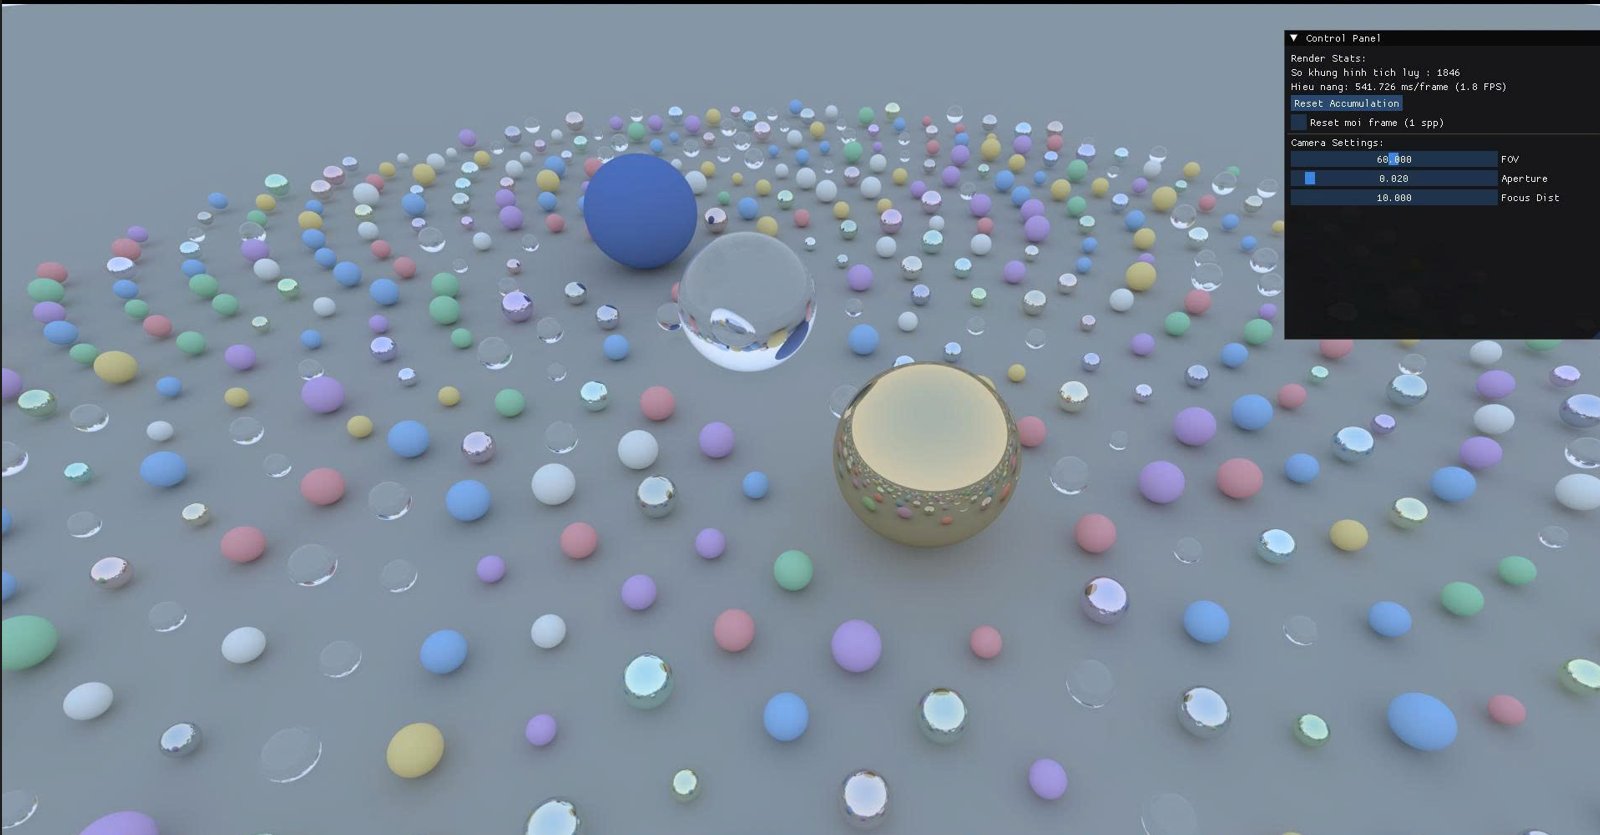
\includegraphics[width=\textwidth]{images/best_render.png}
  \caption{Ảnh kết xuất trên cảnh mật độ cao sau 1846 khung hình tích lũy.}
  \label{fig:best-render}
\end{figure}

\section{Tái tạo các loại vật liệu}
Hình~\ref{fig:three-materials} kiểm chứng riêng ba loại vật liệu đã hiện thực
trên một cảnh thưa để quan sát rõ từng đặc tính, mỗi loại tương ứng một cơ chế
tán xạ khác nhau. Khối cầu màu đỏ là vật liệu Lambertian: bề mặt khuếch tán lý
tưởng có hàm phản xạ hằng số $f_r=\rho/\pi$, tán xạ ánh sáng đều theo mọi hướng
nên bề mặt sáng đục và không phản chiếu môi trường. Khối cầu trong suốt là vật
liệu điện môi: phần khúc xạ tuân theo định luật Snell~\eqref{eq:snell} bẻ cong tia
qua thân cầu làm đảo ngược ảnh nền, còn tỉ lệ năng lượng phản xạ ở rìa tăng vọt
theo xấp xỉ Schlick $R(\theta)=R_0+(1-R_0)(1-\cos\theta)^5$~\eqref{eq:schlick} —
đó là lý do viền cầu sáng và phản chiếu rõ hơn phần giữa. Khối cầu vàng kim là
vật liệu kim loại: tia phản xạ gương quanh pháp tuyến theo
$\mathbf{r}=\mathbf{d}-2(\mathbf{d}\cdot\mathbf{n})\mathbf{n}$~\eqref{eq:reflect}
nên bề mặt ánh lên hình ảnh các vật thể xung quanh. Tại cấu hình khẩu độ bằng 0,
toàn ảnh sắc nét và hệ thống đạt khoảng 57\,ms mỗi khung tương ứng 17{,}5 khung
hình trên giây nhờ số lượng vật thể ít.

\begin{figure}[H]
  \centering
  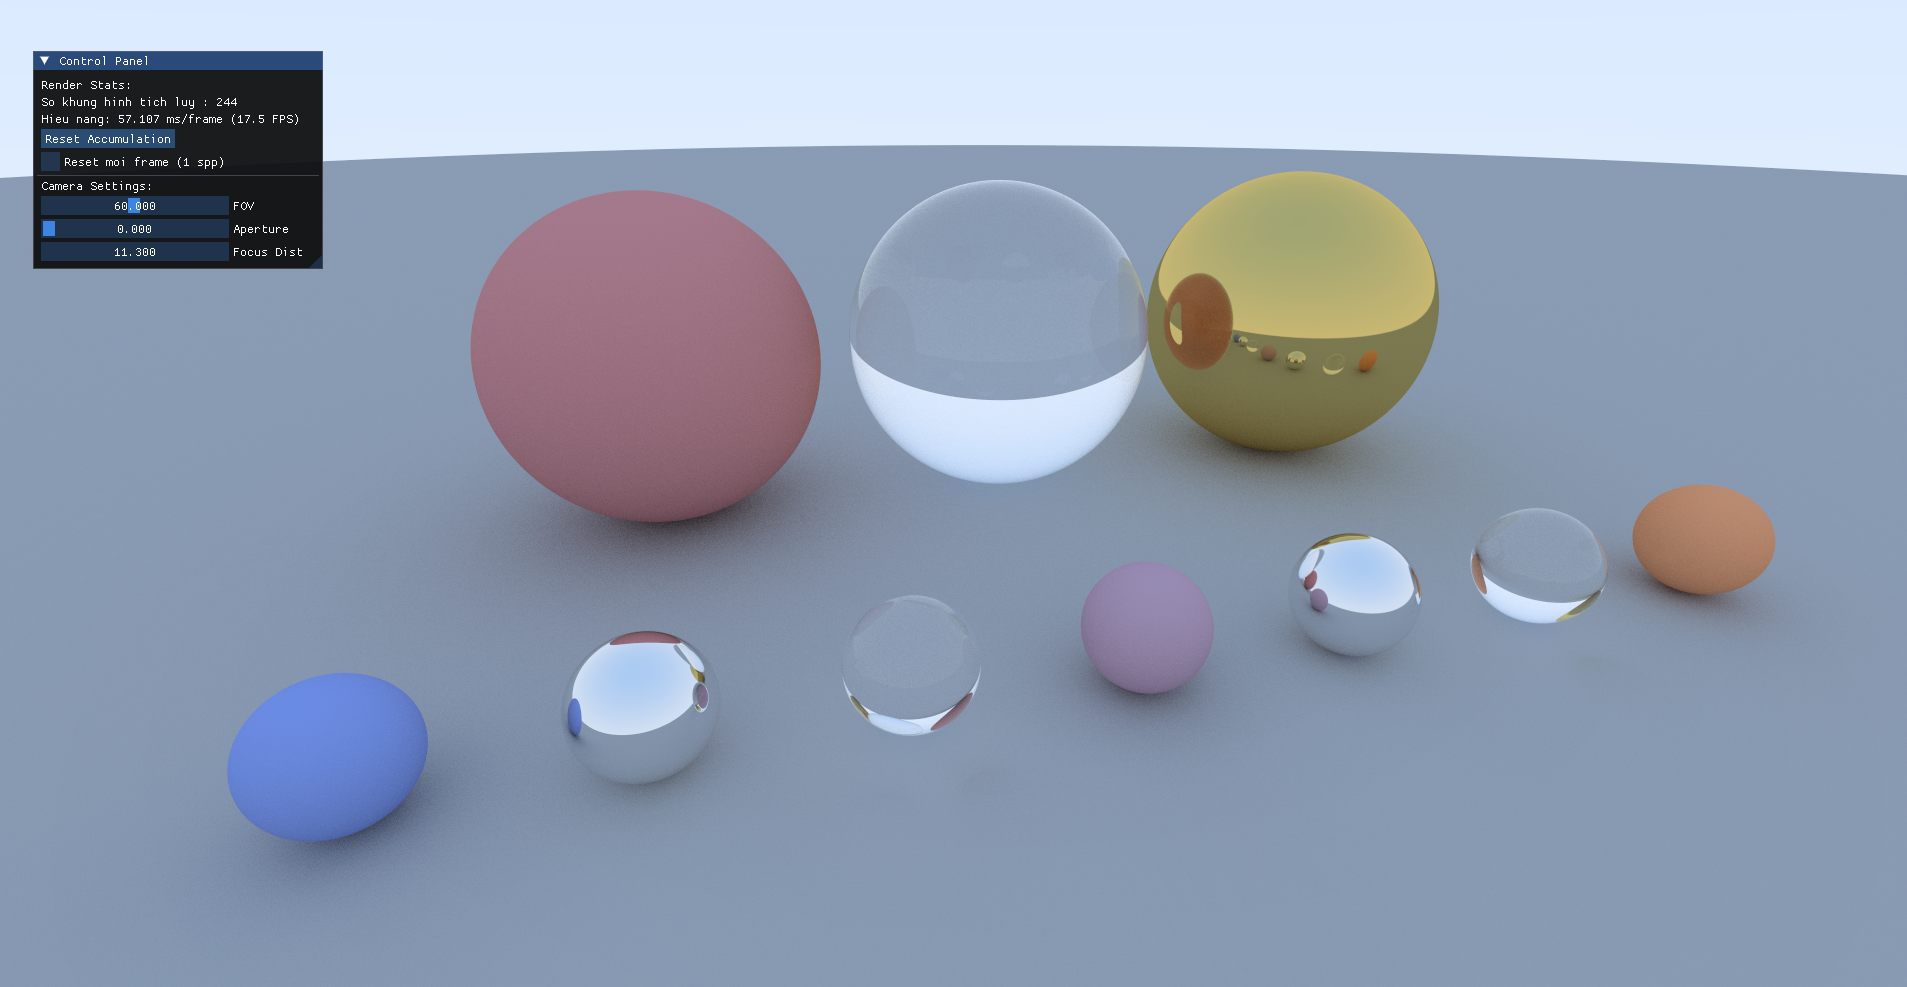
\includegraphics[width=\textwidth]{images/three_materials.png}
  \caption{Ba loại vật liệu Lambertian, điện môi và kim loại trên cùng một cảnh.}
  \label{fig:three-materials}
\end{figure}

\section{Độ sâu trường ảnh}
Hình~\ref{fig:dof} minh họa hai mức khẩu độ khác nhau. Nguyên lý cốt lõi của hiệu
ứng này là khẩu độ hữu hạn của mô hình thấu kính mỏng: mỗi tia không xuất phát từ
một điểm mà từ một vị trí lấy mẫu ngẫu nhiên trên đĩa thấu kính bán kính
$R=\text{khẩu độ}/2$, và mọi tia đều buộc đi qua cùng một điểm trên mặt phẳng lấy
nét. Nhờ vậy vật nằm đúng mặt phẳng lấy nét luôn hội tụ thành một điểm sắc nét;
còn vật ở trước hoặc sau mặt phẳng đó nhận các tia đến từ những vị trí thấu kính
khác nhau nên trải ra thành một đĩa gọi là vòng tròn nhòe. Bán kính vòng nhòe —
và do đó mức độ mờ — tỉ lệ thuận với bán kính khẩu độ $R$: đó là lý do khẩu độ
càng lớn thì vùng rõ nét càng hẹp và hậu cảnh càng mờ. Hiệu ứng phát sinh tự
nhiên từ việc lấy mẫu trên đĩa thấu kính, không cần xử lý hậu kỳ; khi khẩu độ
bằng 0 mô hình thoái biến về camera lỗ kim và toàn ảnh sắc nét.

\begin{figure}[H]
  \centering
  \begin{subfigure}{0.49\textwidth}
    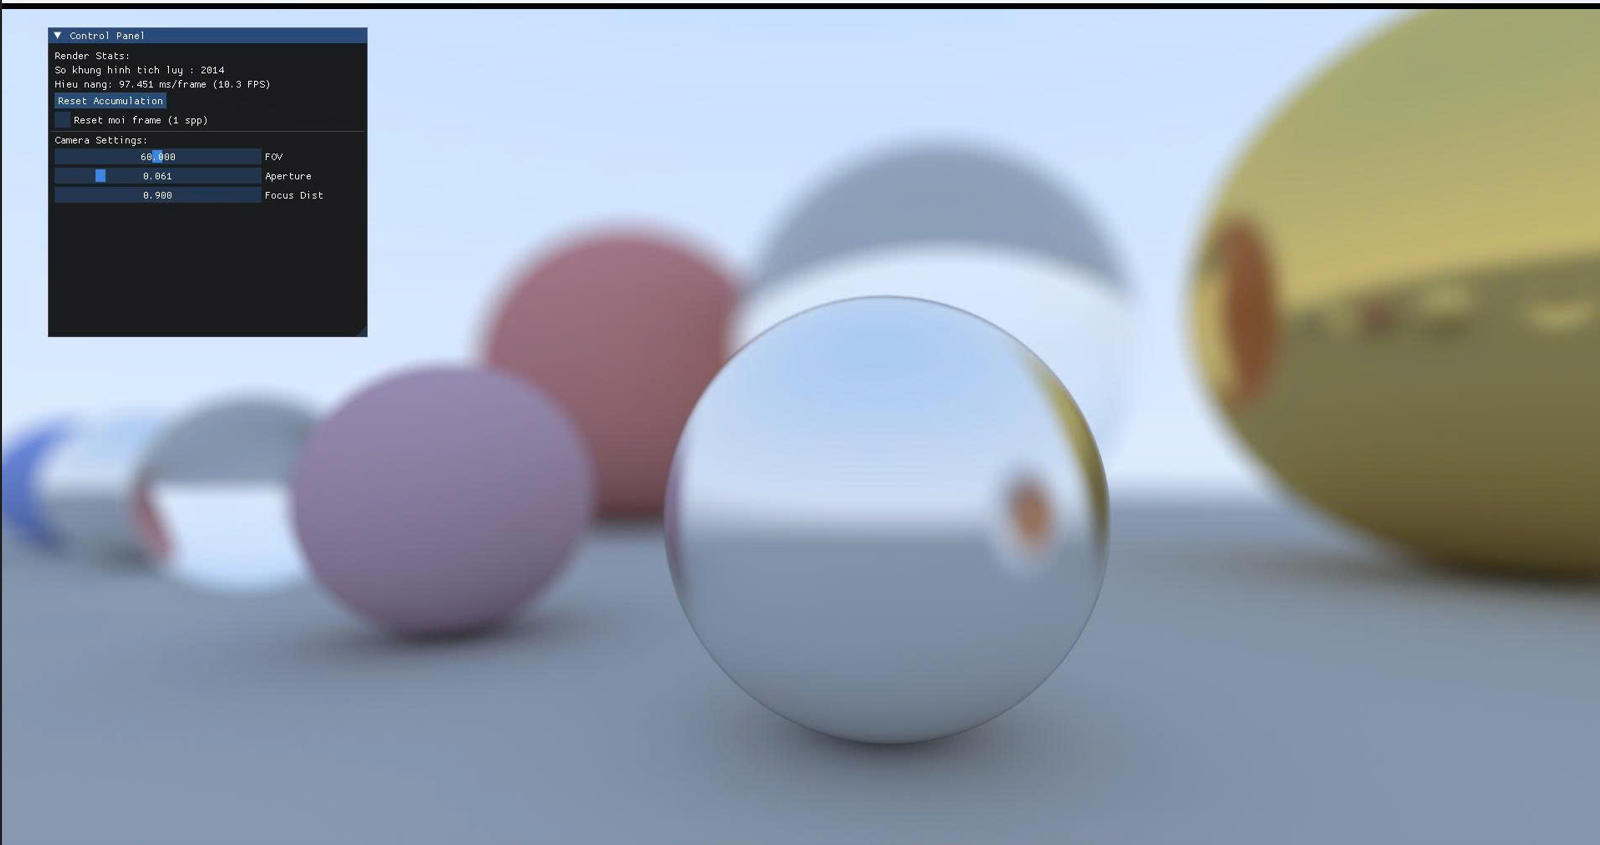
\includegraphics[width=\textwidth]{images/dof_01.png}
    \caption{Khẩu độ 0{,}061, khoảng lấy nét 0{,}9.}
  \end{subfigure}
  \hfill
  \begin{subfigure}{0.49\textwidth}
    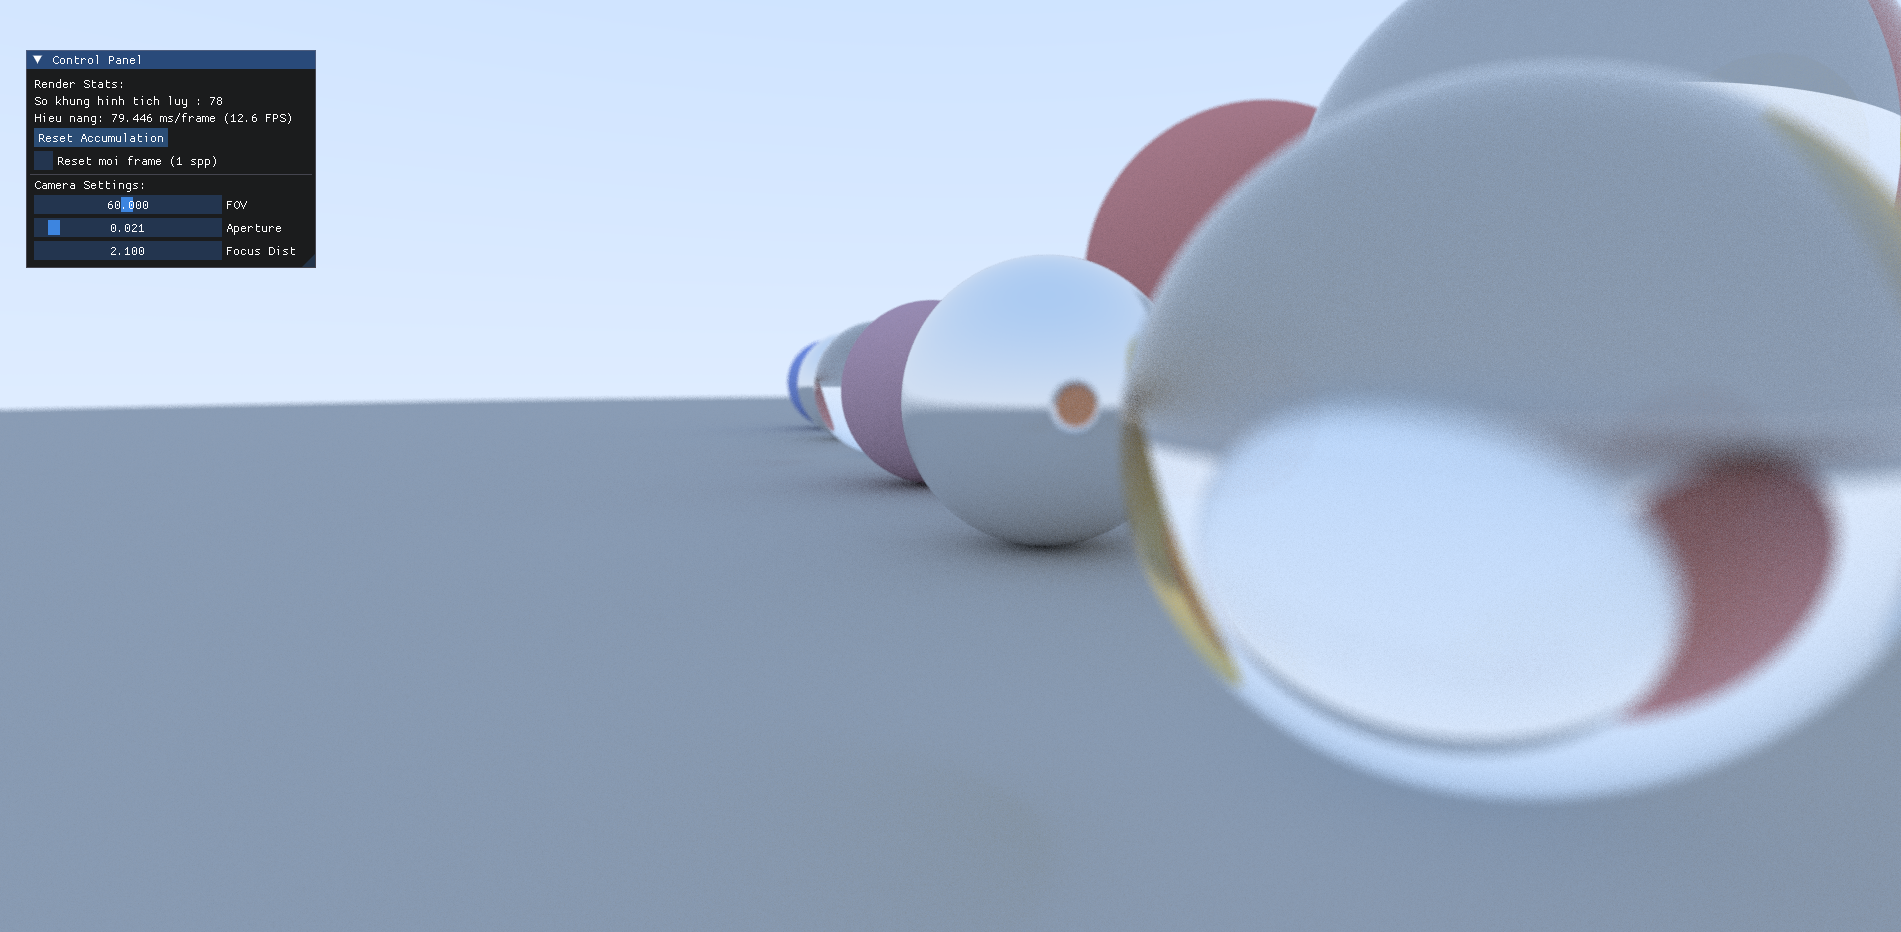
\includegraphics[width=\textwidth]{images/dof_02.png}
    \caption{Khẩu độ 0{,}021, khoảng lấy nét 2{,}1.}
  \end{subfigure}
  \caption{Hiệu ứng độ sâu trường ảnh ở hai cấu hình khẩu độ và khoảng lấy nét.}
  \label{fig:dof}
\end{figure}

\section{Nhòe chuyển động}
Hình~\ref{fig:motion-blur} kiểm chứng hiệu ứng nhòe chuyển động trên cảnh có một
số khối cầu di chuyển. Nguyên lý cốt lõi là camera phơi sáng trong một khoảng
thời gian hữu hạn: giá trị một điểm ảnh không phải bức xạ tại một thời điểm mà là
tích phân của bức xạ theo suốt thời gian màn trập mở $[t_0,t_1]$. Hệ thống ước
lượng tích phân thời gian này bằng Monte Carlo — mỗi tia mang một mốc thời gian
ngẫu nhiên $t\in[t_0,t_1]$, và vị trí khối cầu chuyển động được nội suy tuyến tính
$\mathbf{p}(t)=\mathbf{p}_0+t\,\mathbf{v}$ theo đúng mốc đó. Vì trong một lần phơi
sáng vật đã dịch qua cả quãng đường, năng lượng của nó trải đều dọc quỹ đạo thay
vì đọng tại một chỗ, tạo thành vệt nhòe liên tục; màn trập mở càng lâu (khoảng
$t_1-t_0$ càng lớn) thì vệt nhòe càng dài. Các khối cầu tĩnh không đổi vị trí
theo $t$ nên vẫn sắc nét.

\begin{figure}[H]
  \centering
  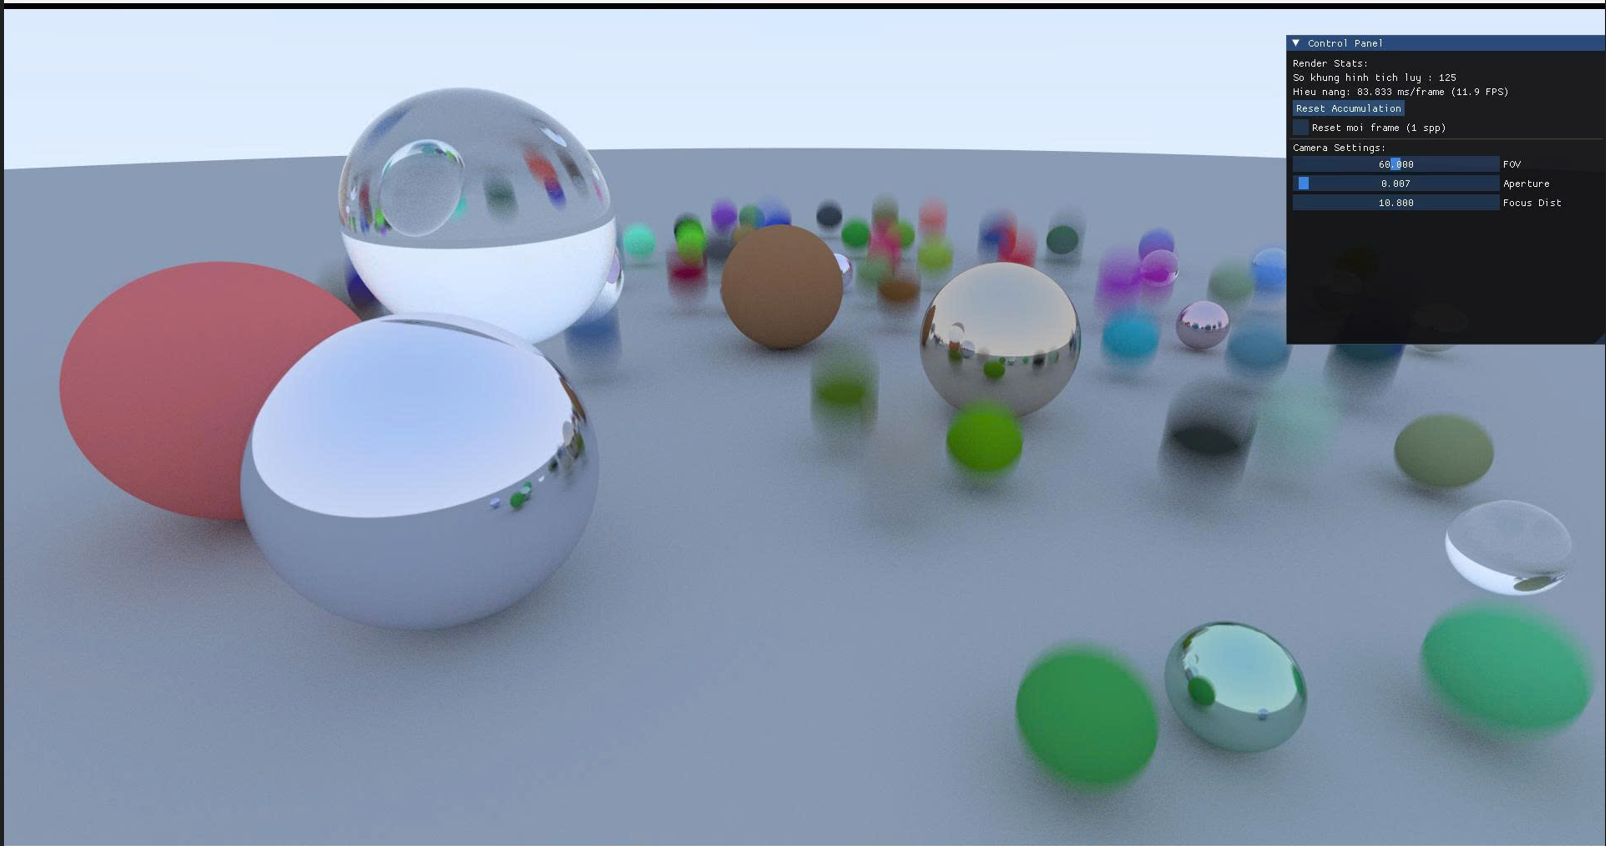
\includegraphics[width=\textwidth]{images/motion_blur.png}
  \caption{Nhòe chuyển động trên các khối cầu được gán vận tốc.}
  \label{fig:motion-blur}
\end{figure}

\section{Làm tối rìa ảnh (Vignetting)}
Hình~\ref{fig:vignette} minh họa hiệu ứng làm tối rìa ảnh áp dụng lên cảnh nhiều
vật liệu. Nguyên lý cốt lõi mà hiệu ứng này mô phỏng là định luật $\cos^4$ của
quang học ống kính: độ rọi tại một điểm trên phim lệch góc $\theta$ so với trục
quang giảm theo
\begin{equation}
\label{eq:cos4}
E(\theta) = E_0 \cos^4\theta,
\end{equation}
trong đó $E_0$ là độ rọi tại tâm ảnh. Số mũ 4 đến từ tích của bốn thừa số cosine:
khoảng cách từ thấu kính tới điểm ảnh xa hơn ở rìa đóng góp $\cos^2\theta$ theo
luật nghịch đảo bình phương, khẩu độ nhìn xiên nên diện tích chiếu giảm thêm
$\cos\theta$, và bề mặt phim nghiêng so với tia tới góp nốt $\cos\theta$. Vì
$\cos\theta$ giảm nhanh khi ra xa trục, độ sáng tụt mạnh ở bốn góc trong khi tâm
ảnh gần như không đổi. Hệ thống tái hiện quy luật này như một bước hậu xử lý điều
khiển bằng tham số Vignette: giá trị càng lớn thì vùng tối ở rìa càng rõ và mở
rộng vào trong, giúp hướng thị giác người xem vào chủ thể ở trung tâm.

\begin{figure}[H]
  \centering
  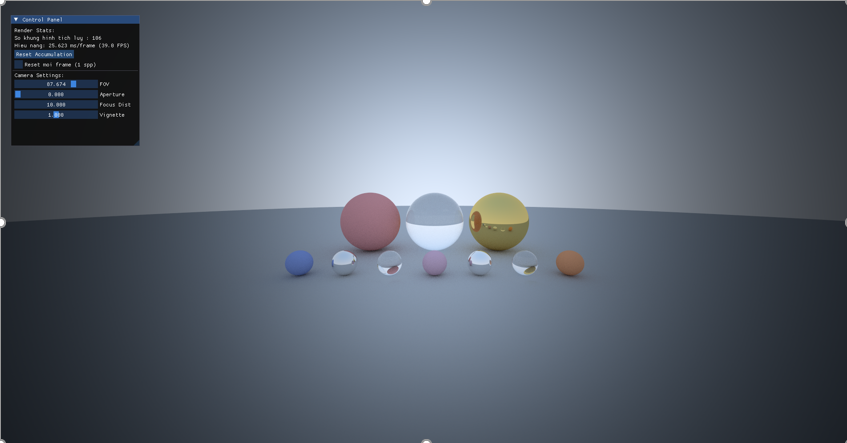
\includegraphics[width=\textwidth]{images/vignette.png}
  \caption{Hiệu ứng làm tối rìa ảnh (vignetting): độ sáng giảm dần từ tâm ra các góc khung hình.}
  \label{fig:vignette}
\end{figure}

\section{Nhận xét chung}
Qua các thử nghiệm trên, hệ thống tái tạo đầy đủ những hiệu ứng quang học mục
tiêu gồm phản xạ, khúc xạ, đổ bóng mềm, độ sâu trường ảnh và nhòe chuyển động,
với chất lượng hình ảnh hội tụ tốt sau vài trăm đến vài nghìn khung hình tích
lũy. Về hiệu năng, hệ thống duy trì tốc độ tương tác từ 10 đến 18 khung hình
trên giây với cảnh thưa, nhưng giảm rõ rệt khi mật độ vật thể tăng cao do chi phí
tìm giao điểm theo phương pháp duyệt tuyến tính. Kết quả này xác nhận tính đúng
đắn của hệ thống đồng thời chỉ ra nút thắt hiệu năng cần được giải quyết bằng cấu
trúc tăng tốc không gian, sẽ được bàn ở Chương~\ref{ch:ket-luan}.

% !TEX root = ../main.tex
%==============================================================
\chapter{Kết luận và hướng phát triển}
\label{ch:ket-luan}

\section{Kết luận}
Đề tài đã nghiên cứu và xây dựng thành công một bộ kết xuất Path Tracing chạy
song song trên kiến trúc CUDA của NVIDIA, đạt được các mục tiêu đề ra ở
Chương~\ref{ch:gioi-thieu}. Cụ thể, hệ thống đã:
\begin{itemize}[noitemsep]
  \item Hiện thực trọn vẹn thuật toán Path Tracing trên GPU bằng CUDA, với vòng
        dò đường theo kiểu lặp và cơ chế tích lũy mẫu theo thời gian để khử
        nhiễu Monte Carlo.
  \item Xây dựng hệ thống vật liệu Lambertian, kim loại và điện môi cùng mô hình
        camera vật lý hỗ trợ độ sâu trường ảnh và nhòe chuyển động.
  \item Hiển thị thời gian thực nhờ cầu nối CUDA--OpenGL, tránh chi phí sao chép
        dữ liệu ảnh qua lại giữa CPU và GPU.
  \item Nạp cảnh theo định dạng Mitsuba~3 và cung cấp giao diện điều khiển tương
        tác để tinh chỉnh camera cũng như theo dõi hiệu năng.
\end{itemize}

Kết quả thực nghiệm ở Chương~\ref{ch:danh-gia} xác nhận hệ thống tái tạo đầy đủ
các hiệu ứng quang học mục tiêu và duy trì tốc độ tương tác trên phần cứng phổ
thông. Đồng thời, thực nghiệm cũng chỉ ra nút thắt hiệu năng khi mật độ vật thể
tăng cao, do việc tìm giao điểm còn thực hiện bằng duyệt tuyến tính, mở ra các
hướng phát triển tiếp theo.

\section{Hướng phát triển}
Trên nền tảng hiện có, hệ thống có thể được mở rộng theo các hướng sau:
\begin{enumerate}[noitemsep]
  \item \textbf{Bounding Volume Hierarchy (BVH):} xây dựng cấu trúc tăng tốc
        không gian để giảm chi phí tìm giao điểm từ tuyến tính xuống mức
        logarit, khắc phục nút thắt hiệu năng ở cảnh mật độ cao.
  \item \textbf{1D/2D:} bổ sung các loại hình học và nguyên thủy một, hai chiều
        (đoạn thẳng, mặt phẳng, tam giác) bên cạnh khối cầu hiện tại.
  \item \textbf{Texture Mapping:} hỗ trợ ánh xạ vân bề mặt để tăng độ chi tiết
        và chân thực cho vật liệu.
  \item \textbf{Emission Material:} thêm vật liệu phát sáng để mô phỏng nguồn
        sáng vùng trực tiếp trong cảnh.
  \item \textbf{Volume Rendering:} kết xuất môi trường tham gia (khói, sương,
        chất bán trong suốt) bằng mô hình tán xạ thể tích.
  \item \textbf{Monte Carlo:} nâng cao chất lượng ước lượng Monte Carlo bằng lấy
        mẫu theo tầm quan trọng (Importance Sampling) và ước lượng sự kiện kế
        tiếp để giảm nhiễu nhanh hơn.
\end{enumerate}

\section{Mã nguồn}
Toàn bộ mã nguồn của đề tài được công khai tại kho lưu trữ:
\begin{center}
\url{https://github.com/KinhLupNe/Path-tracing-Render-CUDA}
\end{center}


%--------- TÀI LIỆU THAM KHẢO ---------
\nocite{*}                               % hiển thị mọi mục trong references.bib
\bibliographystyle{plain}
\bibliography{references}
\addcontentsline{toc}{chapter}{Tài liệu tham khảo}

\end{document}
